\chapter{Experimental Testing}
\label{chap:Experimental Testing}

\section{Velocity Mapping vs. Backwards Difference}
\label{sec:Velocity Mapping vs Backwards Difference}

A number of numeric approximations exist for calculating the velocity mapping from one co-ordinate system to another. 

In \cref{chap:kinematics} the kinematic equations for the leg system between $[r, \theta]$ and $[\phi_1, \phi_2]$ were shown. The Jacobian was also calculated using these kinematic equations.

Two methods for calculating the radial and rotational velocity of the leg foot were used and experimentally tested. 

The first method, using the backwards difference approximation, can be seen in \cref{eq:backwards-difference-approximation}, where $i$ is the sample point index and $t_s$ is the sample time of $5\ ms$. This equation relies on the fact that we know the radial and rotational distance of the foot using the kinematic mapping from Cartesian motor position to polar foot position. 

\begin{equation} \label{eq:backwards-difference-approximation}
\dot{r}(i) = \frac{r(i)-r(i-1)}{t_s}
\end{equation}

The second method, using the Jacobian to map motor velocities to foot velocities, uses the equation derived in \cref{sec:The Jacobian}.

\subsection{Data Analysis}
Initially the backwards difference was used as a quick and simple to implement approximation for velocity. Based on the experimental comparison, in \cref{fig:velocity-calculation}, it was clear to see the Jacobian mapping results in a much more accurate representation of the radial velocity. 

In further experimentation it was found that using the Jacobian derived velocities resulted in a much more smooth spring-damper motion because of the damper force calculation using both radial and rotational velocity calculations. The backwards difference is a relatively inaccurate way of calculating a derivative and was replaced with the Jacobian method for all calculations.

\begin{figure}
\centering
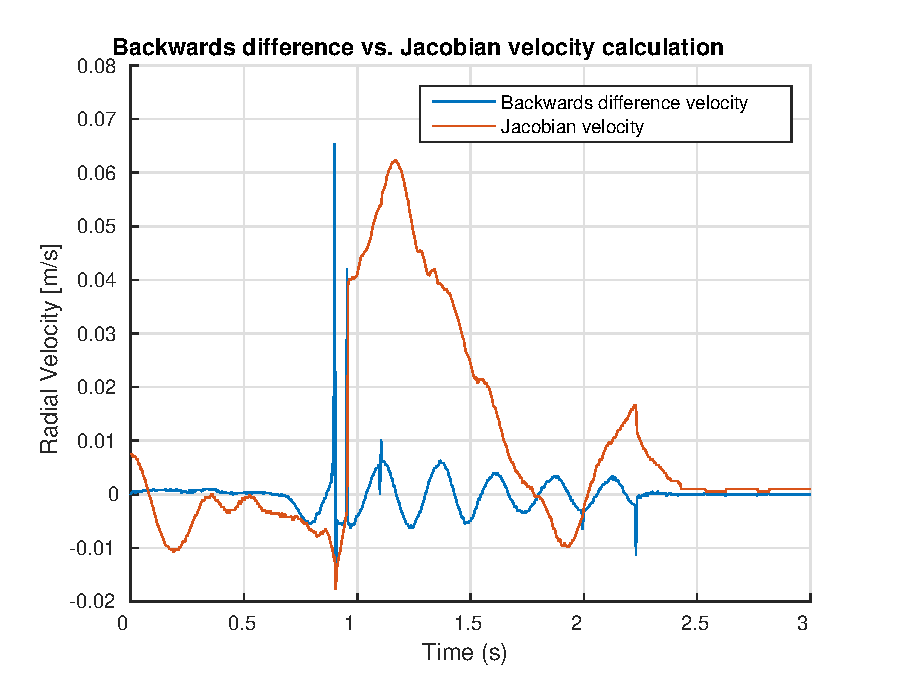
\includegraphics[width=1\textwidth]{images/experiments/velocity-calculation.eps} 
\caption{Comparison of backwards difference and Jacobian velocity calculation methods.}
\label{fig:velocity-calculation}
\end{figure}

\section{Force Control Calibration and Fidelity}
\label{sec:Force Control Calibration and Fidelity}

Force control was implemented by using the relationship between motor torque and the torque constant $K_t$, as developed in \cref{sec:Force Control}. The calibration method was further discussed in \cref{sec:Experimental Calculation of Kt}. 

The following experiment was developed to:
\begin{itemize}
\item Calibrate the torque constant $K_t$ to achieve proprioceptive force control.
\item Validate the transparency of the coupling between the motor torque and the end effector force. 
\item Confirm the linear relationship, with gradient $K_t$, between motor torque and current control input.
\end{itemize}

A load cell was used with a force display. Force values were manually logged while the radial set-point offset $\Delta r$ was changed with the rubber foot placed against the load cell. By varying the radial set-point with the leg firmly attached to the linear guide, the radial set-point offset changes appropriately and the virtual model makes the system behave like a compressed spring with the corresponding force output. 

A virtual compliance model spring constant of $K_s = 200\ N/m$  with zero damping was used which results in the theoretical radial force output derived in \cref{eq:spring-force-equation}.

\begin{equation} \label{eq:spring-force-equation}
F_r = K_s(r_{feedback} - r_{command})
\end{equation}

The theoretical radial force output using \cref{eq:spring-force-equation} was plotted against the force values logged from the load cell. 

\subsection{Experimental Limitations}

In future experimentation a digital load cell capable of continuous logging should be acquired. This was unavailable at the time of testing. The use of a load cell with manual logging meant that only static tests could be performed. In reality we are interested in the dynamic force estimation of the system during jumping. 

The experiment used a limited number of set-point offsets due to logging constraints.

\subsection{Data Analysis}

\Cref{fig:kt-callibration} shows various radial set-point offsets measured during the experiment. Three set points were used, and marked on the plot. 

As can be seen in \cref{fig:kt-callibration-measured}, both the theoretical and measured forces follow a gradient closely matching each other. The theoretical force line crosses the origin, as expected, but the measured force line has an offset of $-5.0156\ N$. By calibrating the torque constant until this offset is zero, we can match the theoretical and measured force measurements for true proprioceptive force control.

\subsection{Summary}

Based on the initial investigative questions, the following results were obtained:
\begin{itemize}
\item \textbf{Calibrate the torque constant $K_t$ to achieve proprioceptive force control:} A value of $K_t = 0.08 Nm/A$ was derived by iterative calibration of the force output. This was confirmed by \cite{Kalouche2016} that determined a value of $K_t = 0.071 Nm/A$.
\item \textbf{Validate the transparency of the coupling between the motor torque and the end effector force:} Both the virtual model estimated force and load cell measured force followed the same gradient, within a margin of experimental error. As expected with a virtual spring constant of $K_s = 200 N/m$ the theoretical force followed a gradient of 200, while the load cell force followed a gradient of $185.54$ - this indicates limited mechanical impedance and dynamic interference between the motor and end effector coupling.
\item \textbf{Confirm the linear relationship, with gradient $K_t$, between motor torque and current control input:} As covered in the previous point, the force gradients were near identical. Both the theoretical and measured force followed a linear pattern which confirms the linear relationship between motor torque and control current! This is sometimes not the case when non-linear dynamics are involved, which once again confirms transparency.
\end{itemize}

\begin{figure}
\centering
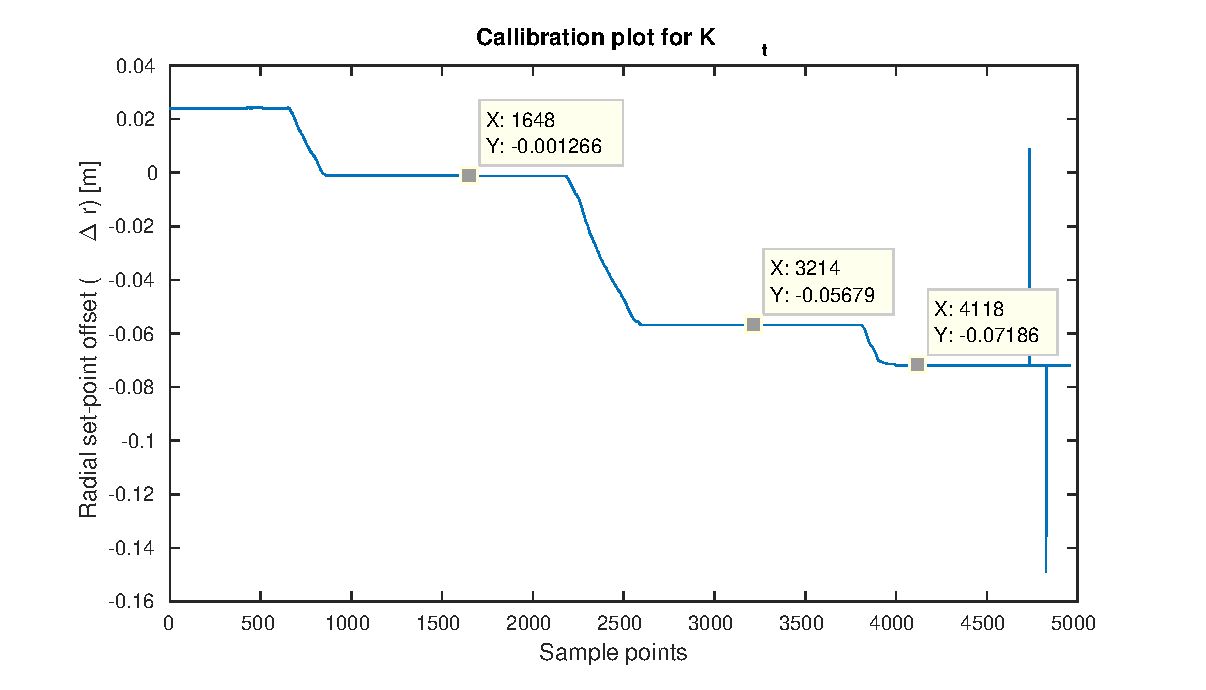
\includegraphics[width=0.8\textwidth]{images/experiments/kt-callibration.eps} 
\caption{Calibration of $K_t$: plot of radial set-point offset over time.}
\label{fig:kt-callibration}
\end{figure}

\begin{figure}
\centering
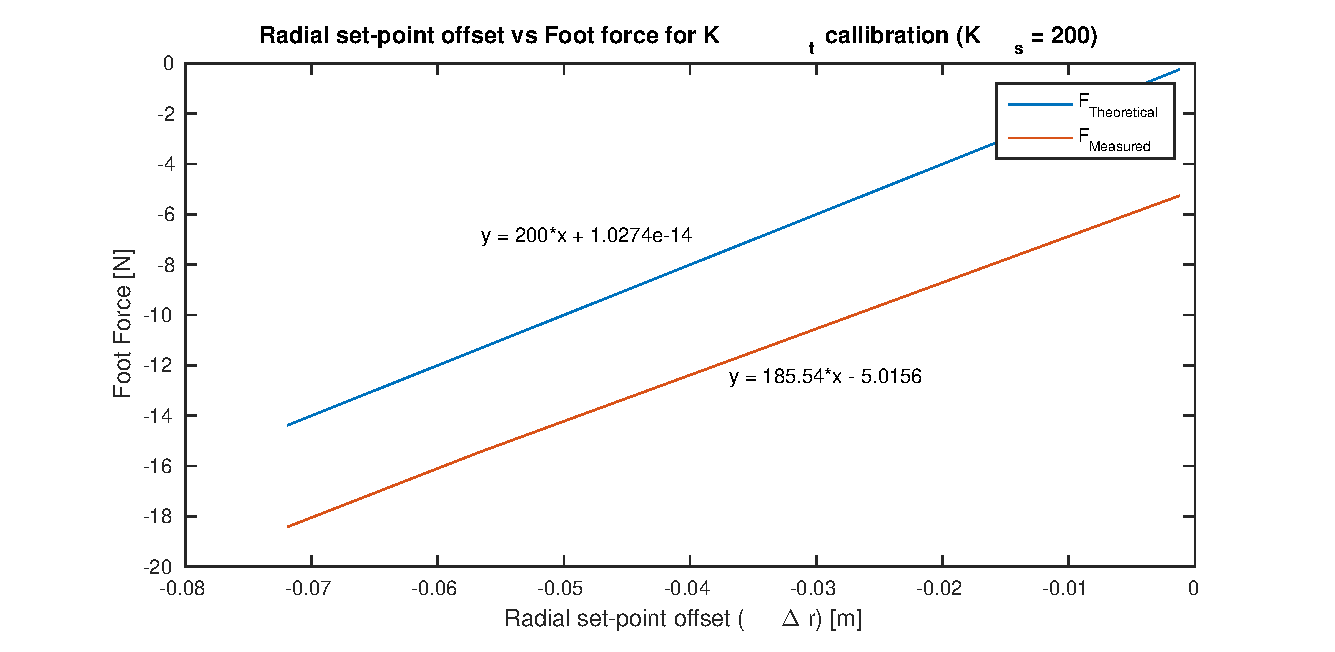
\includegraphics[width=0.8\textwidth]{images/experiments/kt-callibration-measured.eps} 
\caption{Calibration of $K_t$: plot of radial force (theoretical and measured) vs radial set-point offset.}
\label{fig:kt-callibration-measured}
\end{figure}

\section{Virtual Spring-damper Tests} 
\label{sec:Virtual Spring-damper Tests}

The virtual spring-damper model, developed in \cref{chap:Dynamic Modelling} and comprised of a linear and torsional spring-damper, was tested with various constants and in full-leg and joint spring-damper topology.

The experiment aimed to investigate:

\begin{enumerate}
\item Accuracy of theoretical virtual model design versus practical implementation.
\item Ideal spring-damper configuration for leg jump control.
\item Effect of virtual model spring-damper topology on leg dynamics.
\end{enumerate}

The leg was fixed at a height of $0.4\ m$ and allowed to freely move in mid-air. The torsional spring-damper was set to a value of $K_s = 300\ N/m$ and $K_d = 10\ N/(m/s)$ in order to keep the leg from rotating. The purpose of the experiment was to investigate a single spring-damper pair, namely the linear spring damper.

For all tests the radial set-point, $r_0$, was set to $0.3\ m$ and offset by $r_{offset} = r - r_0 = 0.13\ m$ before being released to oscillate. The leg weight was measured as $0.5\ kg$ which served as an approximation for the virtual model mass in mid-air.

\subsection{Full-leg Spring Damper Topology}

The full-leg spring-damper model in \cref{fig:Leg spring-damper virtual model} serves as a reference for the experimentation performed.

Using \cref{eq:natural-freq} to calculate the theoretical natural frequency of oscillation, $\omega_0$, we get:

\begin{equation}
\begin{aligned}
&\text{Spring constant of 100 N/m:}\\
&\omega_0 = \sqrt{\frac{100}{0.5}} = 14.14\ rad/s\\
&\text{Spring constant of 200 N/m:}\\
&\omega_0 = \sqrt{\frac{200}{0.5}} = 20\ rad/s\\
&\text{Spring constant of 300 N/m:}\\
&\omega_0 = \sqrt{\frac{300}{0.5}} = 24.49\ rad/s\\
\end{aligned}
\end{equation}

The experimental natural frequencies were all within a reasonable experimental error of the theoretical values. The natural frequency for a spring constant of $200\ N/m$ and higher seemed to be a higher fidelity representation of the virtual model. This is likely due to the mechanical impedance that exists in the leg design, as discussed in \cref{sec:Mechanical Impedance}, causing the relatively low force experiment for $K_s = 100\ N/m$ to not overcome the deadband that exists. 

The mechanical impedance in question caused the $K_s = 100\ N/m$ foot force to decay rapidly whereas the higher spring constant tests continued to oscillate, thus better representing the virtual model and resulting in a natural frequency much closer to theory.

As the damping increased, the decay rate increased dramatically. For a damping of $K_d = 1\ N/(m/s)$ the damping ratio, $\zeta$, was calculated. This was only calculated for a subset of the plots because the calculations were not theoretically accurate, as discussed in \cref{sec:Spring-Damper-Test:Experimental Limitations}. These damping ratios show a clear relationship between spring constant and damping constant, where \cref{eq:damping-ratio} defines the theoretical relationship. The damping ratio decreases with increasing spring constant, as expected.

The motor control plots in \cref{fig:full-leg-spring-damper-motor-control} show accurate current command set-point tracking, symmetric position and velocity plots and a controlled decay in radial foot force. A maximum motor velocity of $100\ rad/s$ was experienced with a corresponding current command of $20\ A$ a radial foot force of $40\ N$.

\begin{figure}
\centering
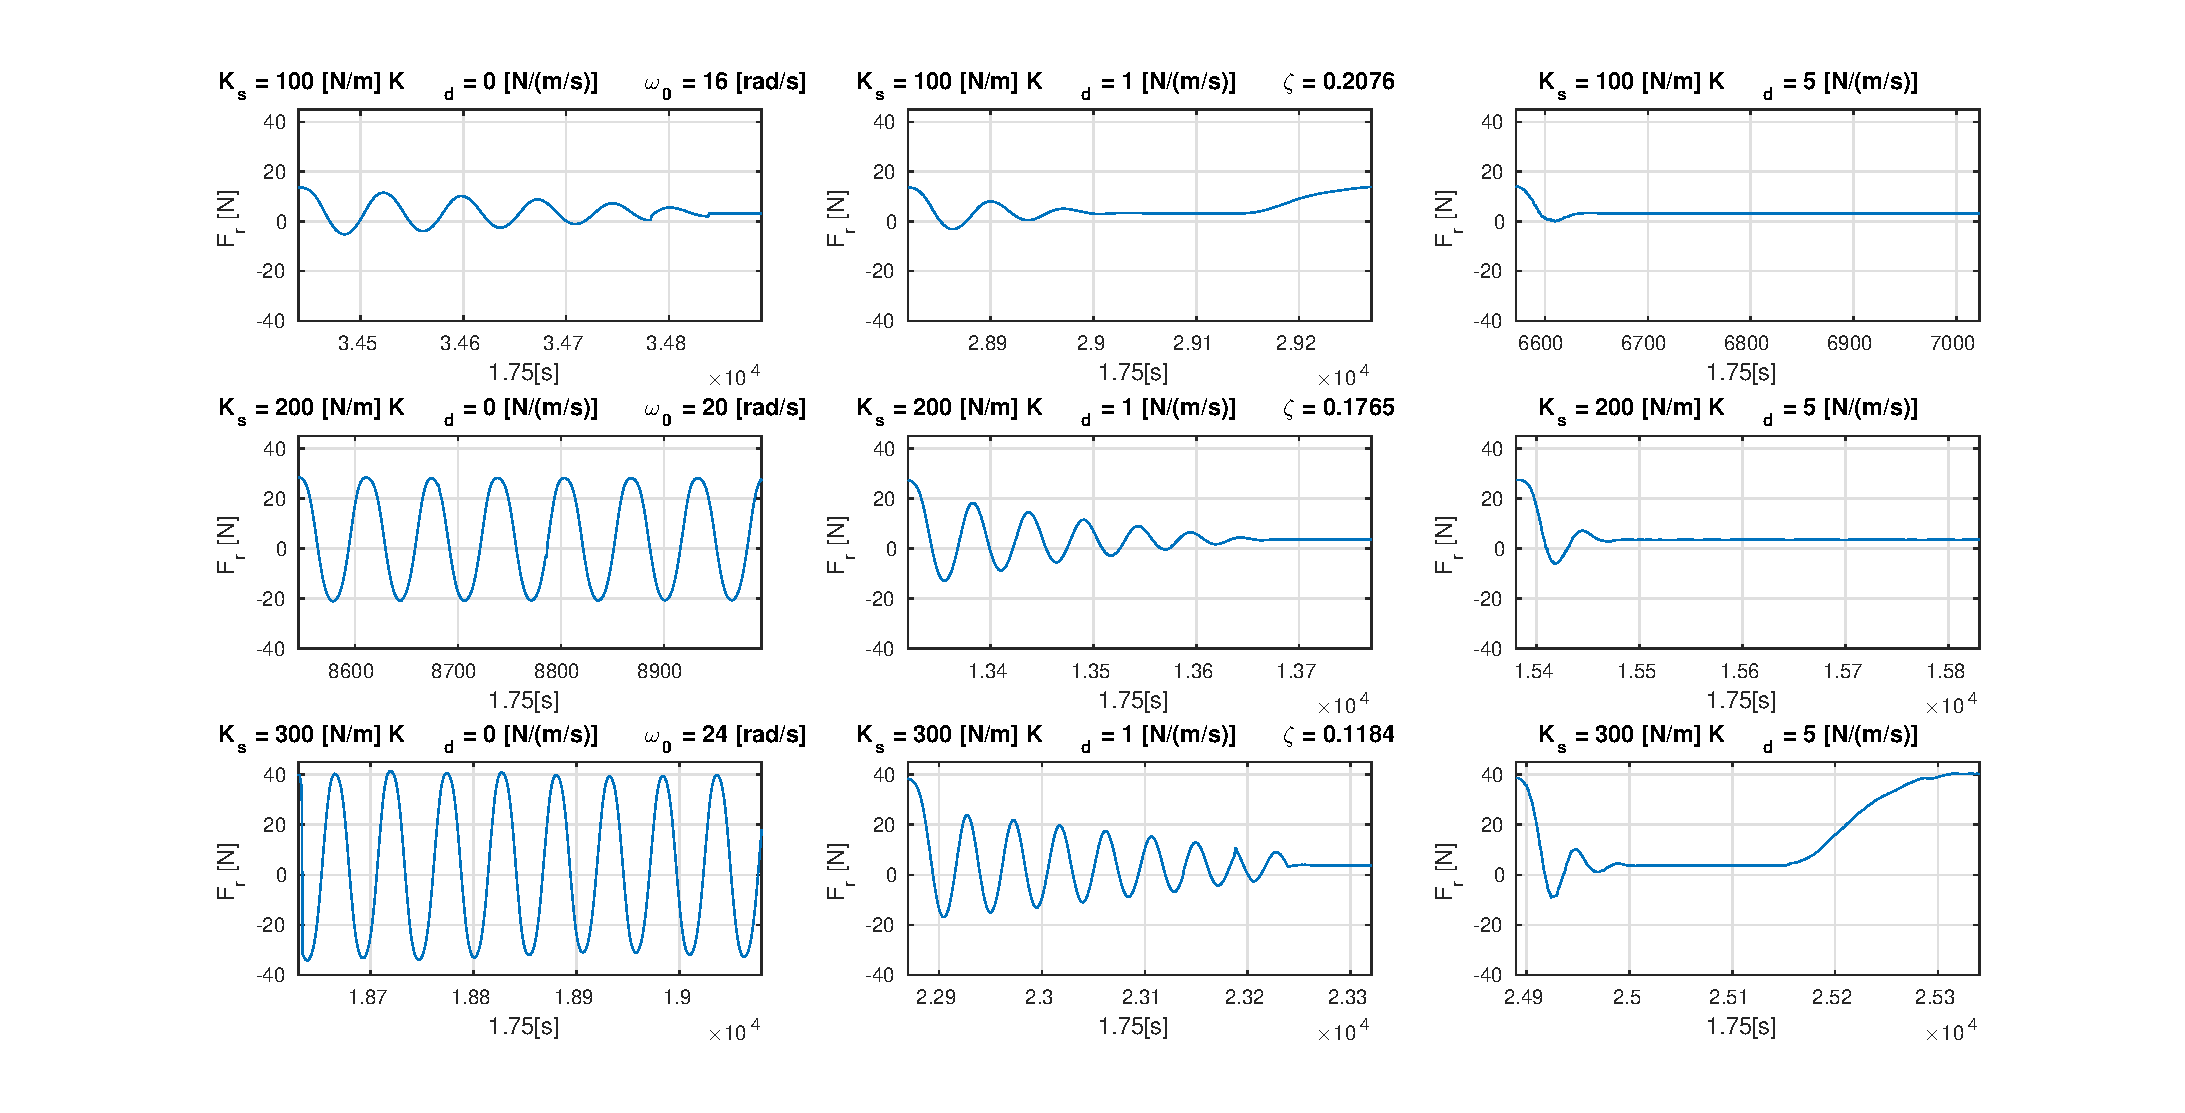
\includegraphics[width=1\textwidth]{images/experiments/spring-damper-tests2.eps} 
\caption{Full-leg spring damper testing for radial offset.}
\label{fig:spring-damper-tests}
\end{figure}

\begin{figure}
\centering
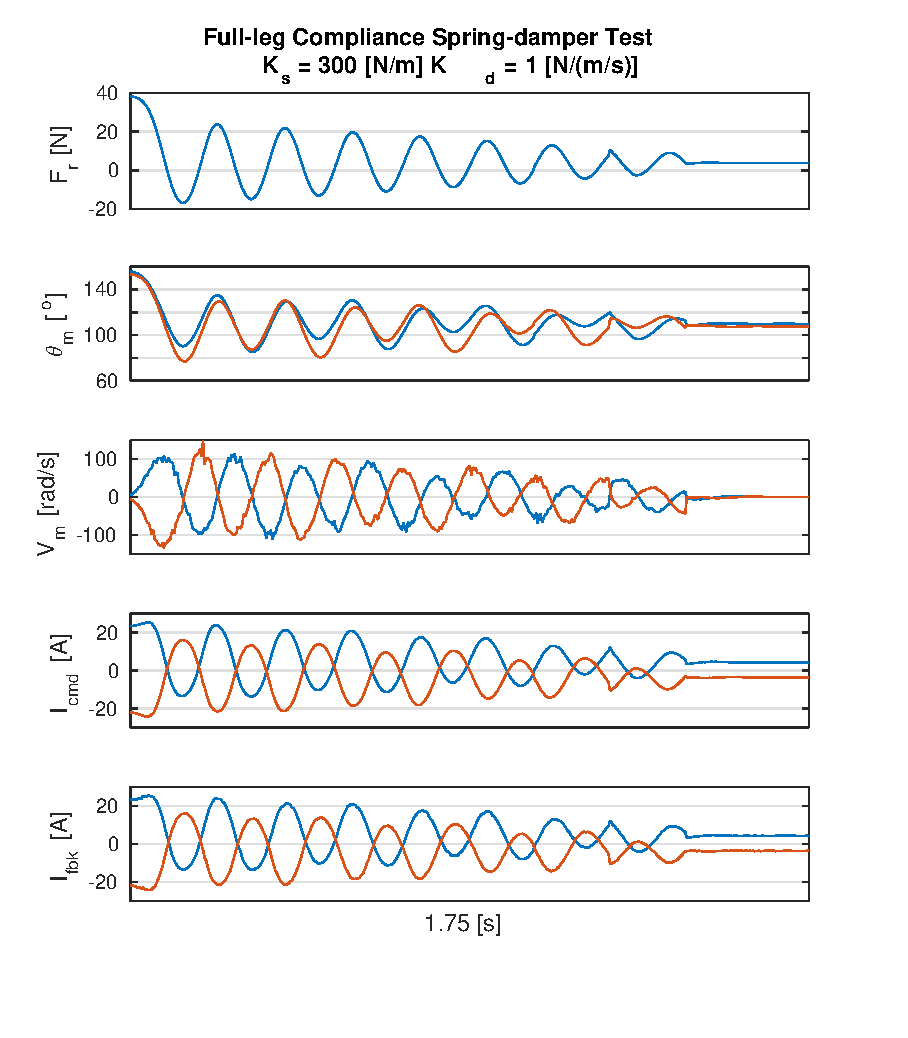
\includegraphics[width=1\textwidth]{images/experiments/full-leg-spring-damper-control-output.eps} 
\caption{Full-leg spring damper motor control.}
\label{fig:full-leg-spring-damper-motor-control}
\end{figure}

\subsection{Joint Spring Damper Topology}

The joint spring-damper model in \cref{fig:Joint spring-damper virtual model} serves as a reference for the experimentation performed.

A scaling factor of $0.01$ was used for the joint compliance model spring and damping constants. This was done so that the constants were effectively normalised, rather than dealing with the small spring and damping constants needed to effect proper control.

Using \cref{eq:natural-freq} to calculate the theoretical natural frequency of oscillation, $\omega_0$, we get:
\begin{equation}
\begin{aligned}
&\text{Spring constant of 300 N/m:}\\
&\omega_0 = \sqrt{\frac{300}{0.5}} = 24.49\ rad/s\\
&\text{Spring constant of 400 N/m:}\\
&\omega_0 = \sqrt{\frac{400}{0.5}} = 28.28\ rad/s\\
\end{aligned}
\end{equation}

The comparison of theoretical and experimental natural frequency is not as clearly defined when dealing with a joint spring damper model, although the experimental natural frequencies were within a reasonable margin of error of the theoretical values.

The motor control plots in \cref{fig:joint-spring-damper-motor-control} show a relatively fast foot force decay with the current command for each motor offset significantly from zero. A maximum motor velocity of $60\ rad/s$ was experienced with a corresponding current command of $20\ A$ a radial foot force of $35\ N$.

\begin{figure}
\centering
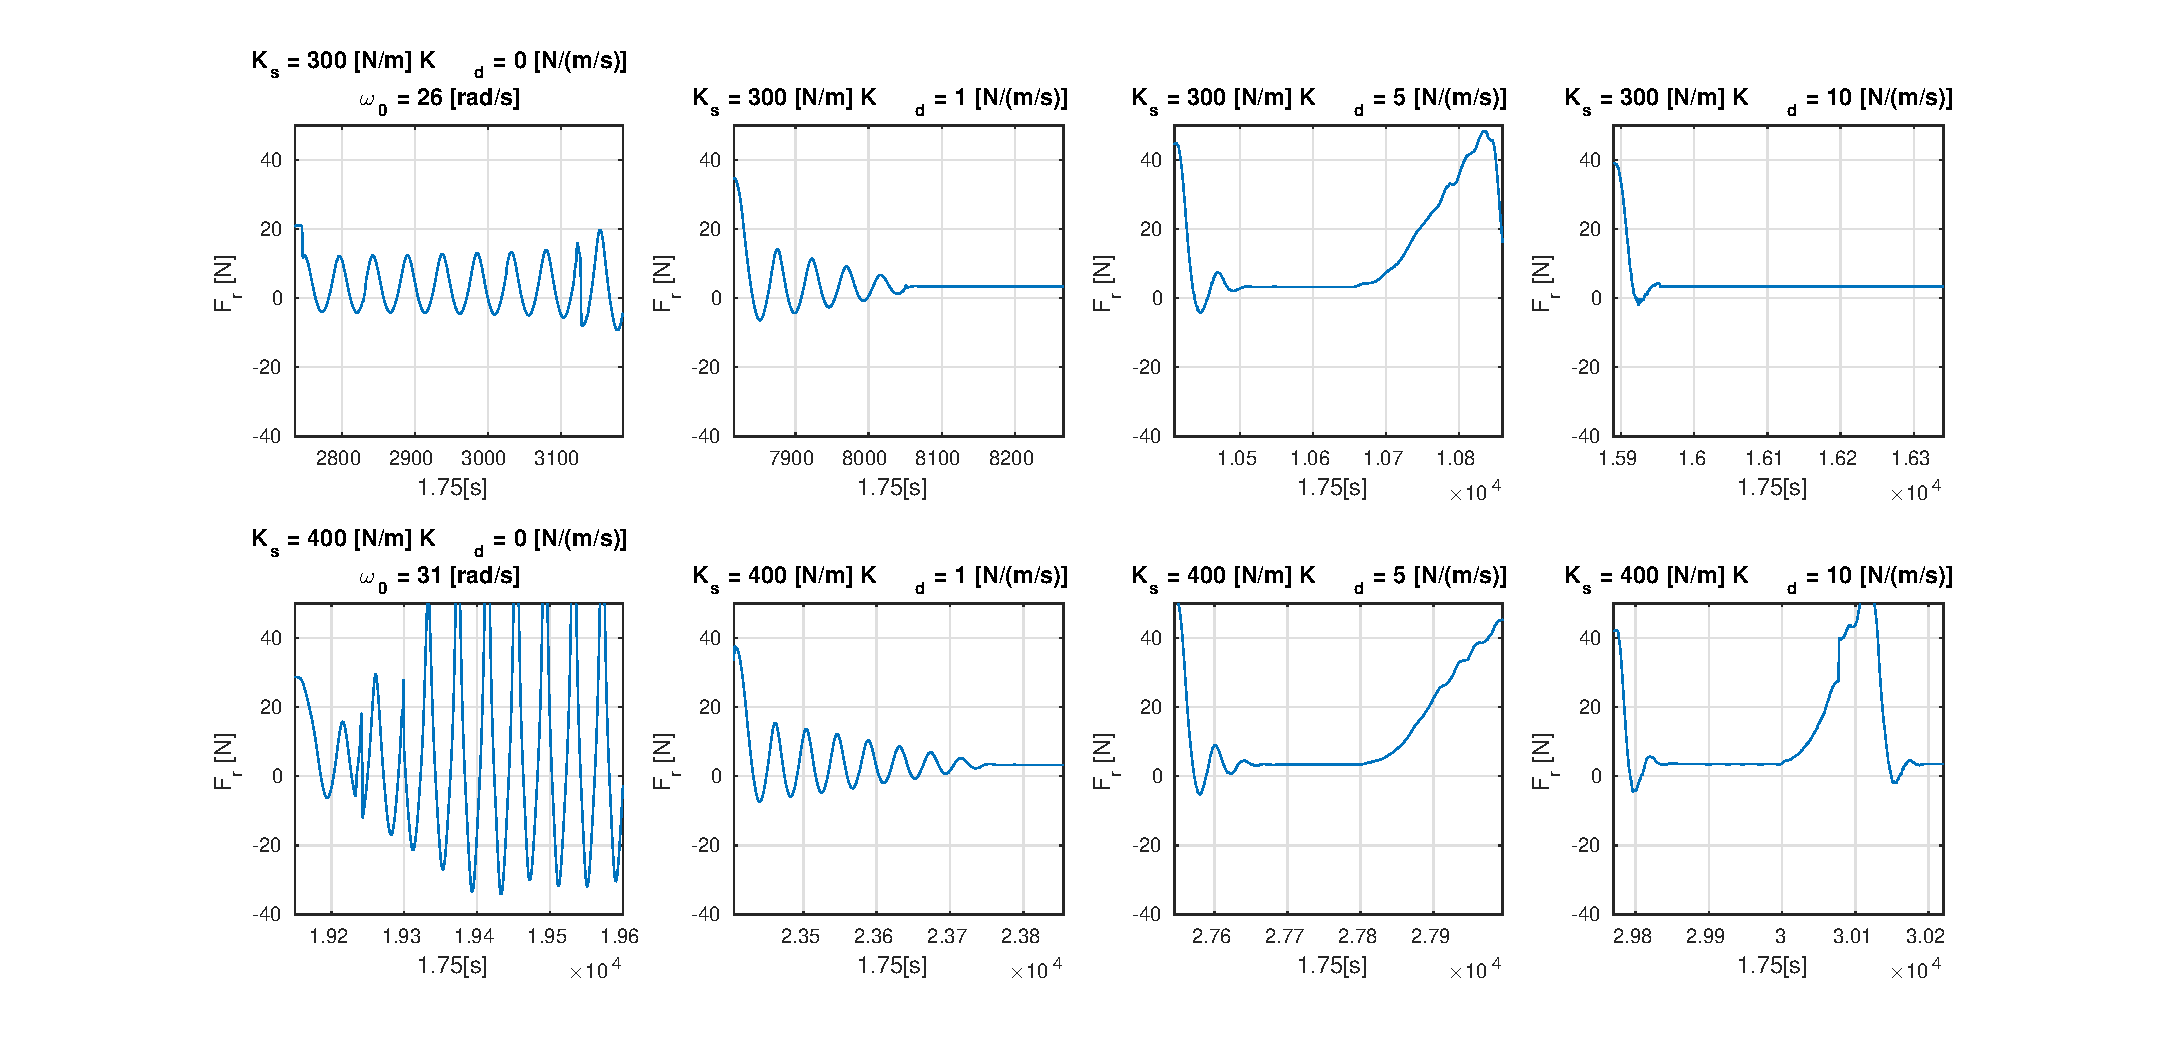
\includegraphics[width=1\textwidth]{images/experiments/joint-spring-damper-tests.eps} 
\caption{Joint spring damper testing for radial offset.}
\label{fig:joint-spring-damper-tests}
\end{figure}

\begin{figure}
\centering
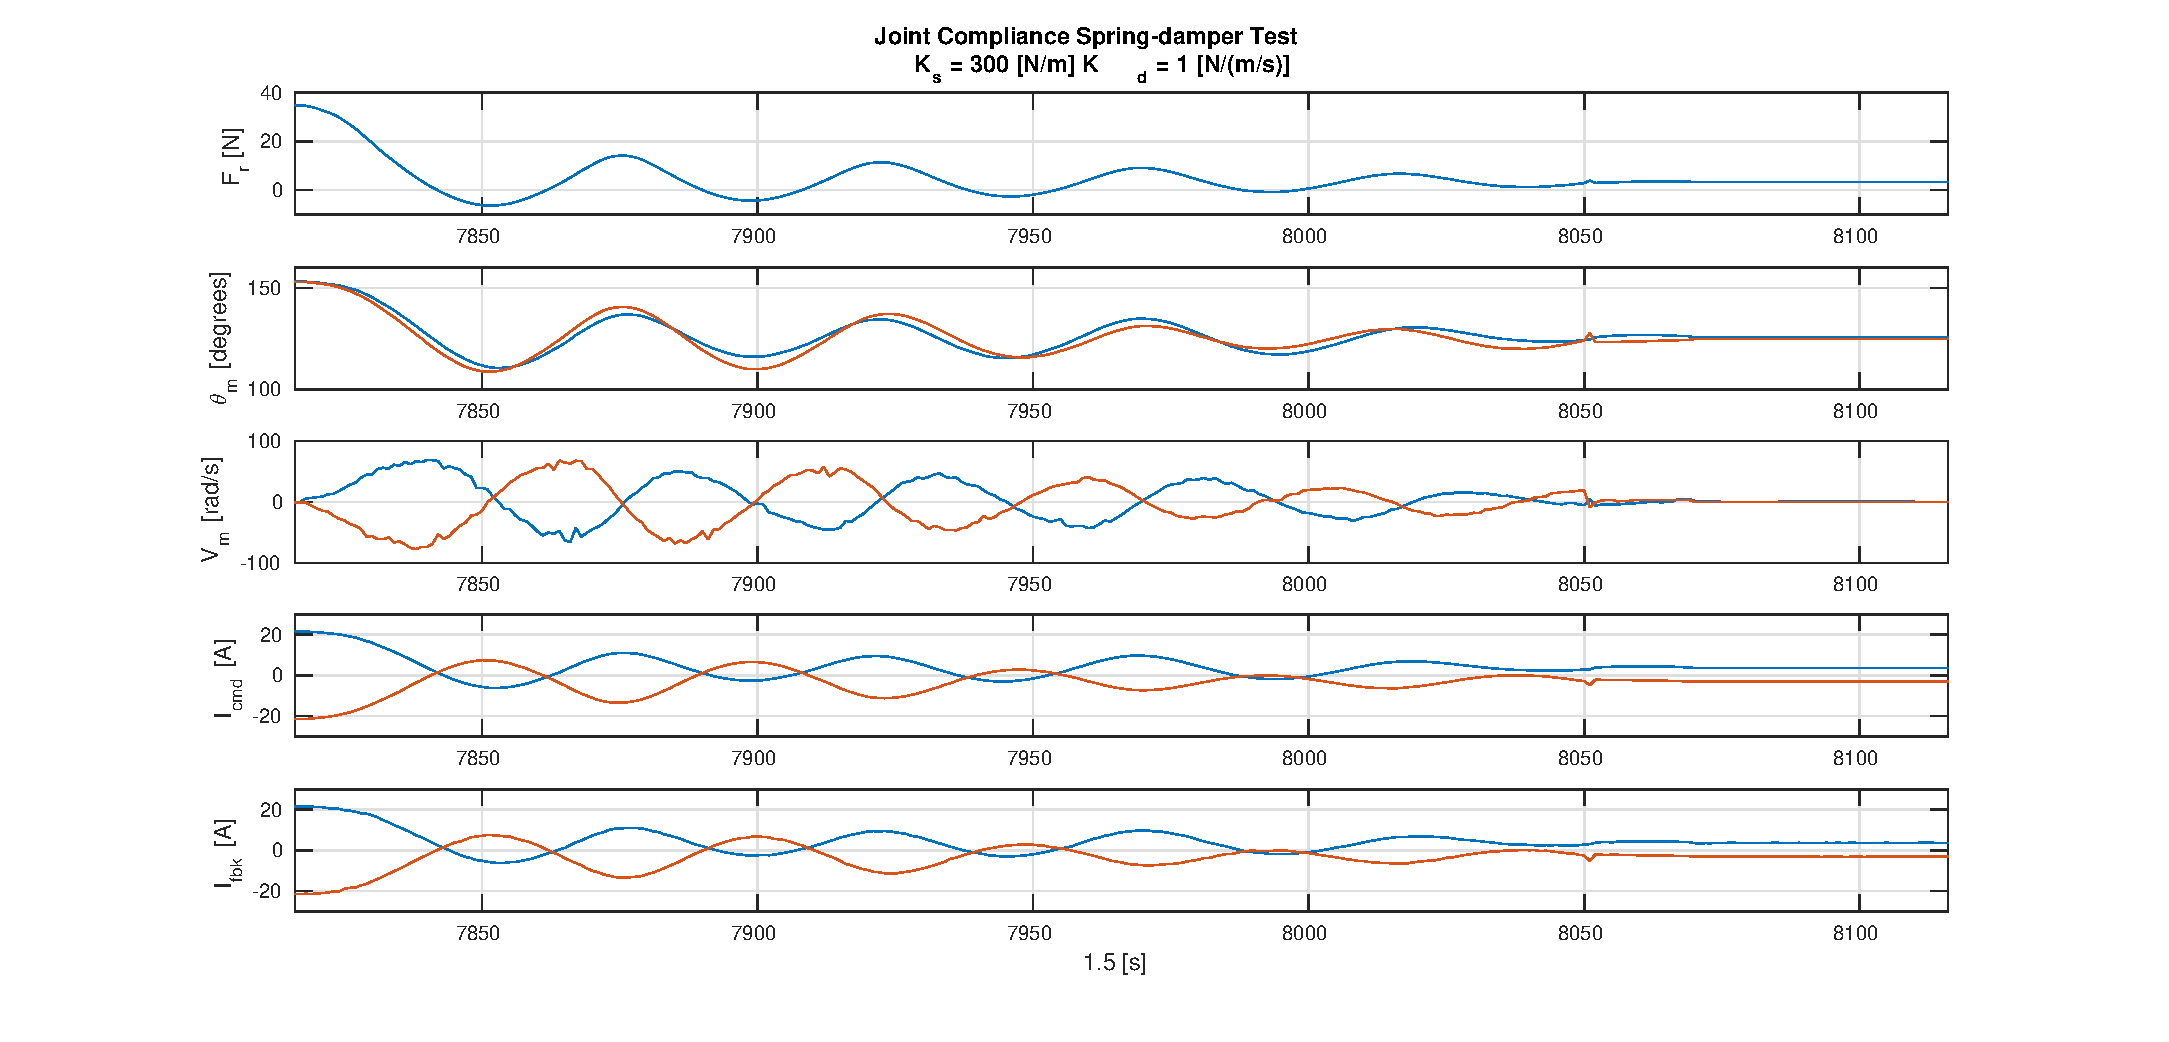
\includegraphics[width=1\textwidth]{images/experiments/joint-spring-damper-control-output.eps} 
\caption{Joint spring damper motor control.}
\label{fig:joint-spring-damper-motor-control}
\end{figure}

\subsection{Experimental Limitations}
\label{sec:Spring-Damper-Test:Experimental Limitations}

The undamped spring tests used to determine the natural frequency were difficult to perform as the leg oscillated unstably. In cases were it looked like the oscillation stopped, this was a case of having to forcibly stop the oscillation in order to prevent any damage to the platform.

The tests were performed before the velocity mapping was improved by using the Jacobian method instead of the backwards difference. This means the damping effect, although visible and functional, was not scientifically accurate when compared with the theoretical calculations. For this reason, the damping ratios were not included for most of the plots. The experiments rather served to theoretically compare natural frequencies, and to practically determine the best configuration for spring-damping during jump control. 

\subsection{Summary}

The following conclusions were made based on the original investigative aims:

\begin{enumerate}
\item \textbf{Accuracy of theoretical virtual model design versus practical implementation:} The natural frequencies measured from the undamped systems closely matched the theoretical values. Damping had the expected effect on oscillations, but was realistically not scientifically sound because of mechanical impedance that exists in the leg design and the use of the backwards difference for velocity mapping.
\item \textbf{Ideal spring-damper configuration for leg jump control:} The ideal spring-damper configuration for reduction of oscillations during flight while maintaining rapid leg position recovery was determined to be approximately $K_s = 300\ N/(m/s)$ and $K_d = 5\ N/(m/s)$.
\item \textbf{Effect of virtual model spring-damper topology on leg dynamics:} Using full-leg spring damper control resulted in a more desirable mid-air motion and a faster recovery.
\end{enumerate}

\section{Drop Tests}
\label{sec:Drop Tests}

The drop test experiments aimed to investigate the leg response to impact and the effect of spring constants and damping on the spring damper mass motion derived in \cref{sec:Spring-damper Mass Motion}. The results of these tests lead to the final choice of spring-damper constants implemented in the virtual model and tested in the jump tests during the landing phase seen in \cref{fig:jump-phases-experiment}.

A theoretical value for the spring constant $K_s$, with $K_d = 5\ N/(m/s)$, for radial spring-damping upon impact was determined in \cref{sec:Leg Spring-damper Model} using conservation of energy and an ideal dynamic response. The calculated spring constant of $632.8\ N/m$ was used as a starting point for testing and the damping was varied from $0\ N/(m/s)$ to $5\ N/(m/s)$ to confirm the values derived.

The drop tests plots of \cref{fig:drop-tests} show a plot of radial foot force versus sample points at $5\ ms$ per sample, with the total plot duration shown for reference.

\subsection{Experimental Limitations}

The drop tests were performed from a maximum height of $0.5\ m$ and as such were limited to a subset of possible drop heights. The linear guide provided significant damping in the form of friction - this must be taken into account when analysing the data. In an ideal experiment the leg would oscillate continuously with zero damping, but in reality the oscillation were damped very quickly.

\subsection{Data Analysis}

With a spring constant of $K_s = 500\ N/m$ a damping constant of $K_d = 10\ N/(m/s)$ resulted in no overshoot, but significant undershoot.

The spring constant of $K_s = 800\ N/m$ served as a practical maximum due to the severe rebound experienced with zero damping - as the leg impacted the ground it oscillated twice mid-air before landing again. A damping value of $K_d = 20\ N/(m/s)$ provided a relatively smooth response with diminishing returns for higher damping constants. 

Theoretically with a spring constant of $K_s = 500\ N/m$, and using the critical damping equation derived in \cref{sec:Spring-damper Mass Motion}, a critical damping constant of $66\ N/(m/s)$ should result in no overshoot. Practically it was not possible to implement a damping constant higher than $30\ N/(m/s)$ as the high frequency noise was amplified, as determined in \cref{eq:derivative-freq-response}, resulting in an unstable system.

\subsection{Summary}

Based on the experimental data analysis, the following conclusions can be made:
\begin{enumerate}
\item The system can adequately dissipate the energy from high speed impacts.
\item The effect of damping can not be fully tested due to its high frequency noise amplification characteristic which causes an unstable system. 
\item The spring-damper virtual model behaves as expected on impact.
\item The spring constant values between $K_s = 500\ N/m$ and an upper limit of $800\ N/m$ can be used for impact absorption during jump experimentation.
\end{enumerate}

\begin{figure}
\centering
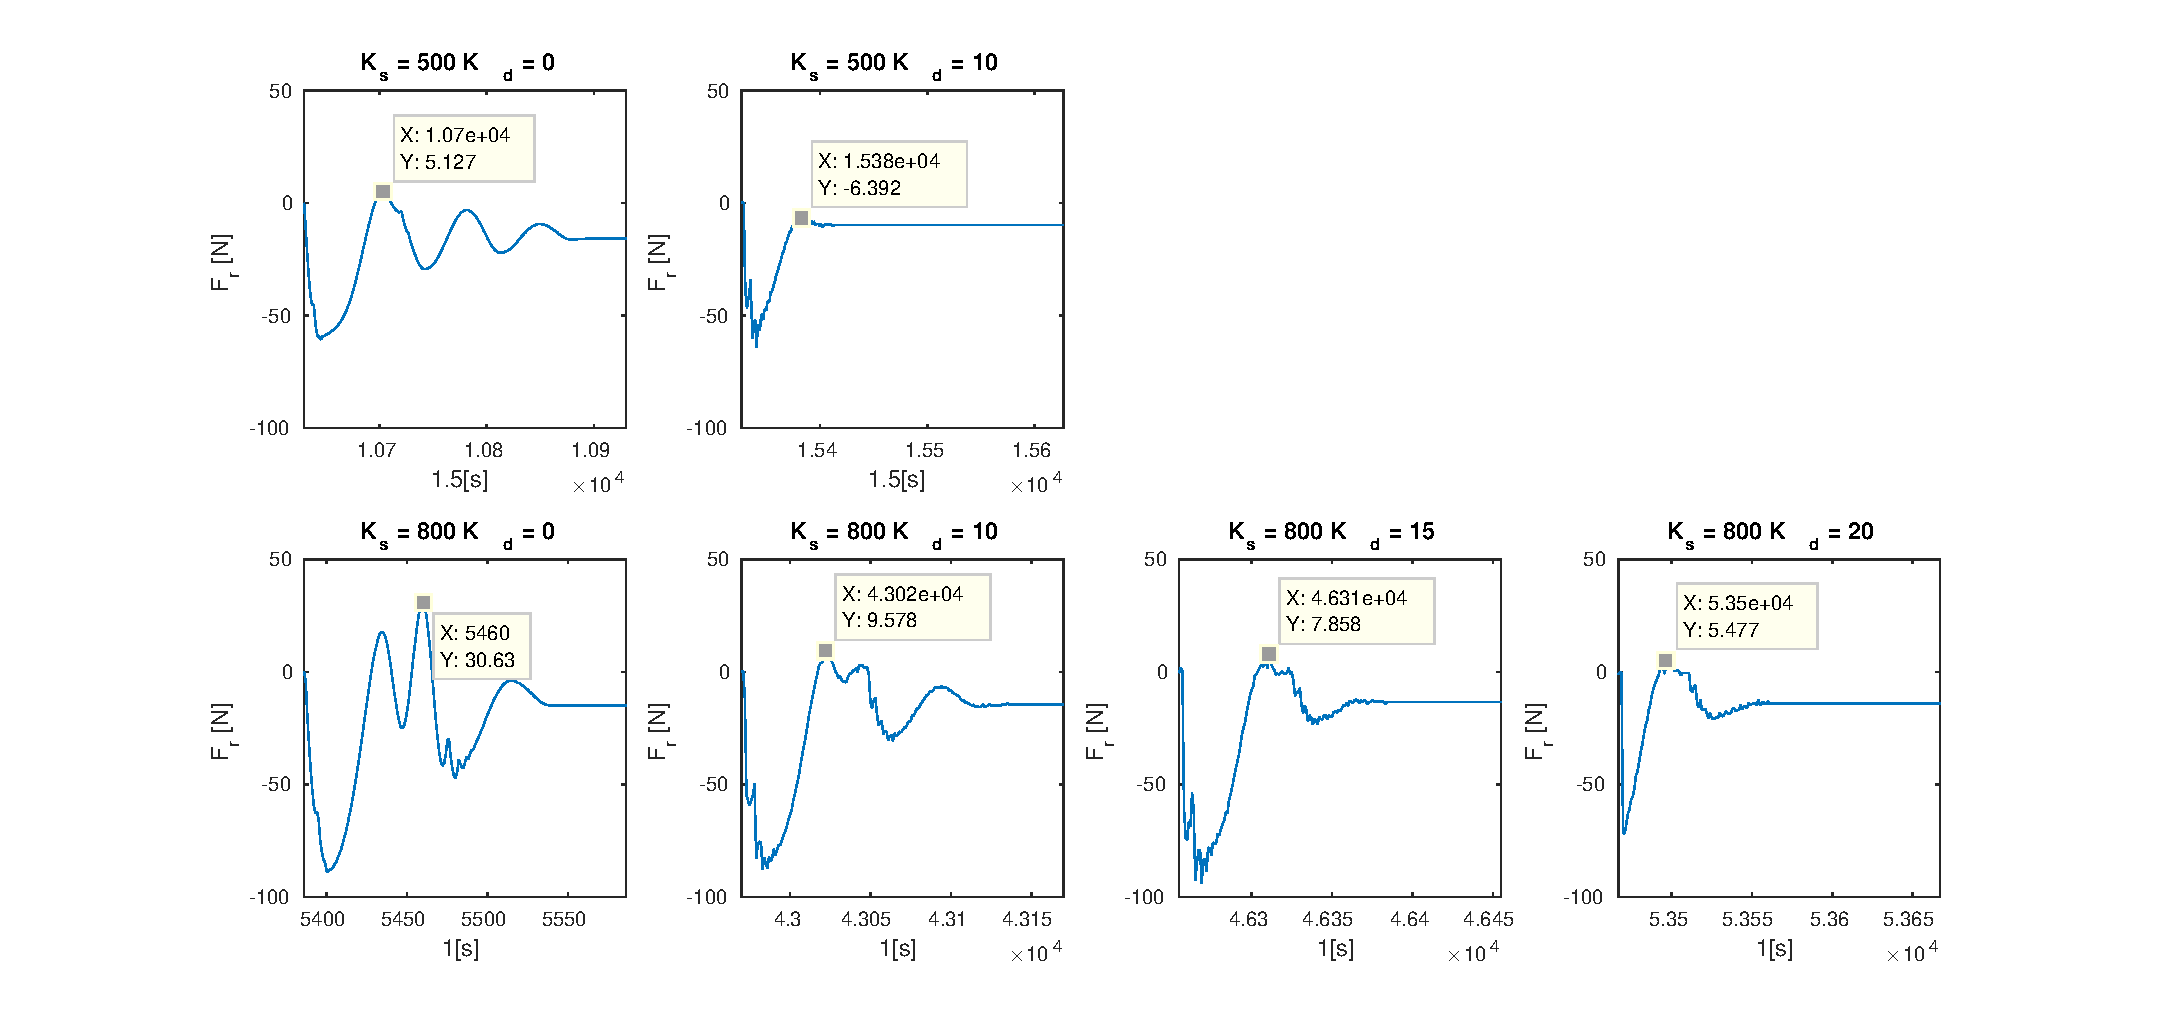
\includegraphics[width=1\textwidth]{images/experiments/drop-test-force-plots.eps} 
\caption{Leg spring damper drop testing.}
\label{fig:drop-tests}
\end{figure}

\section{Jump Test}
\label{sec:Jump Test}

A summary of the jump phases and experimental setup can be seen in \cref{fig:jump-phases-experiment}. The radial foot forces experienced at each jump phase are included as well as the radial and rotational spring-damper constants. The development of this experiment will be expanded upon in more detail.

\begin{figure}
\centering
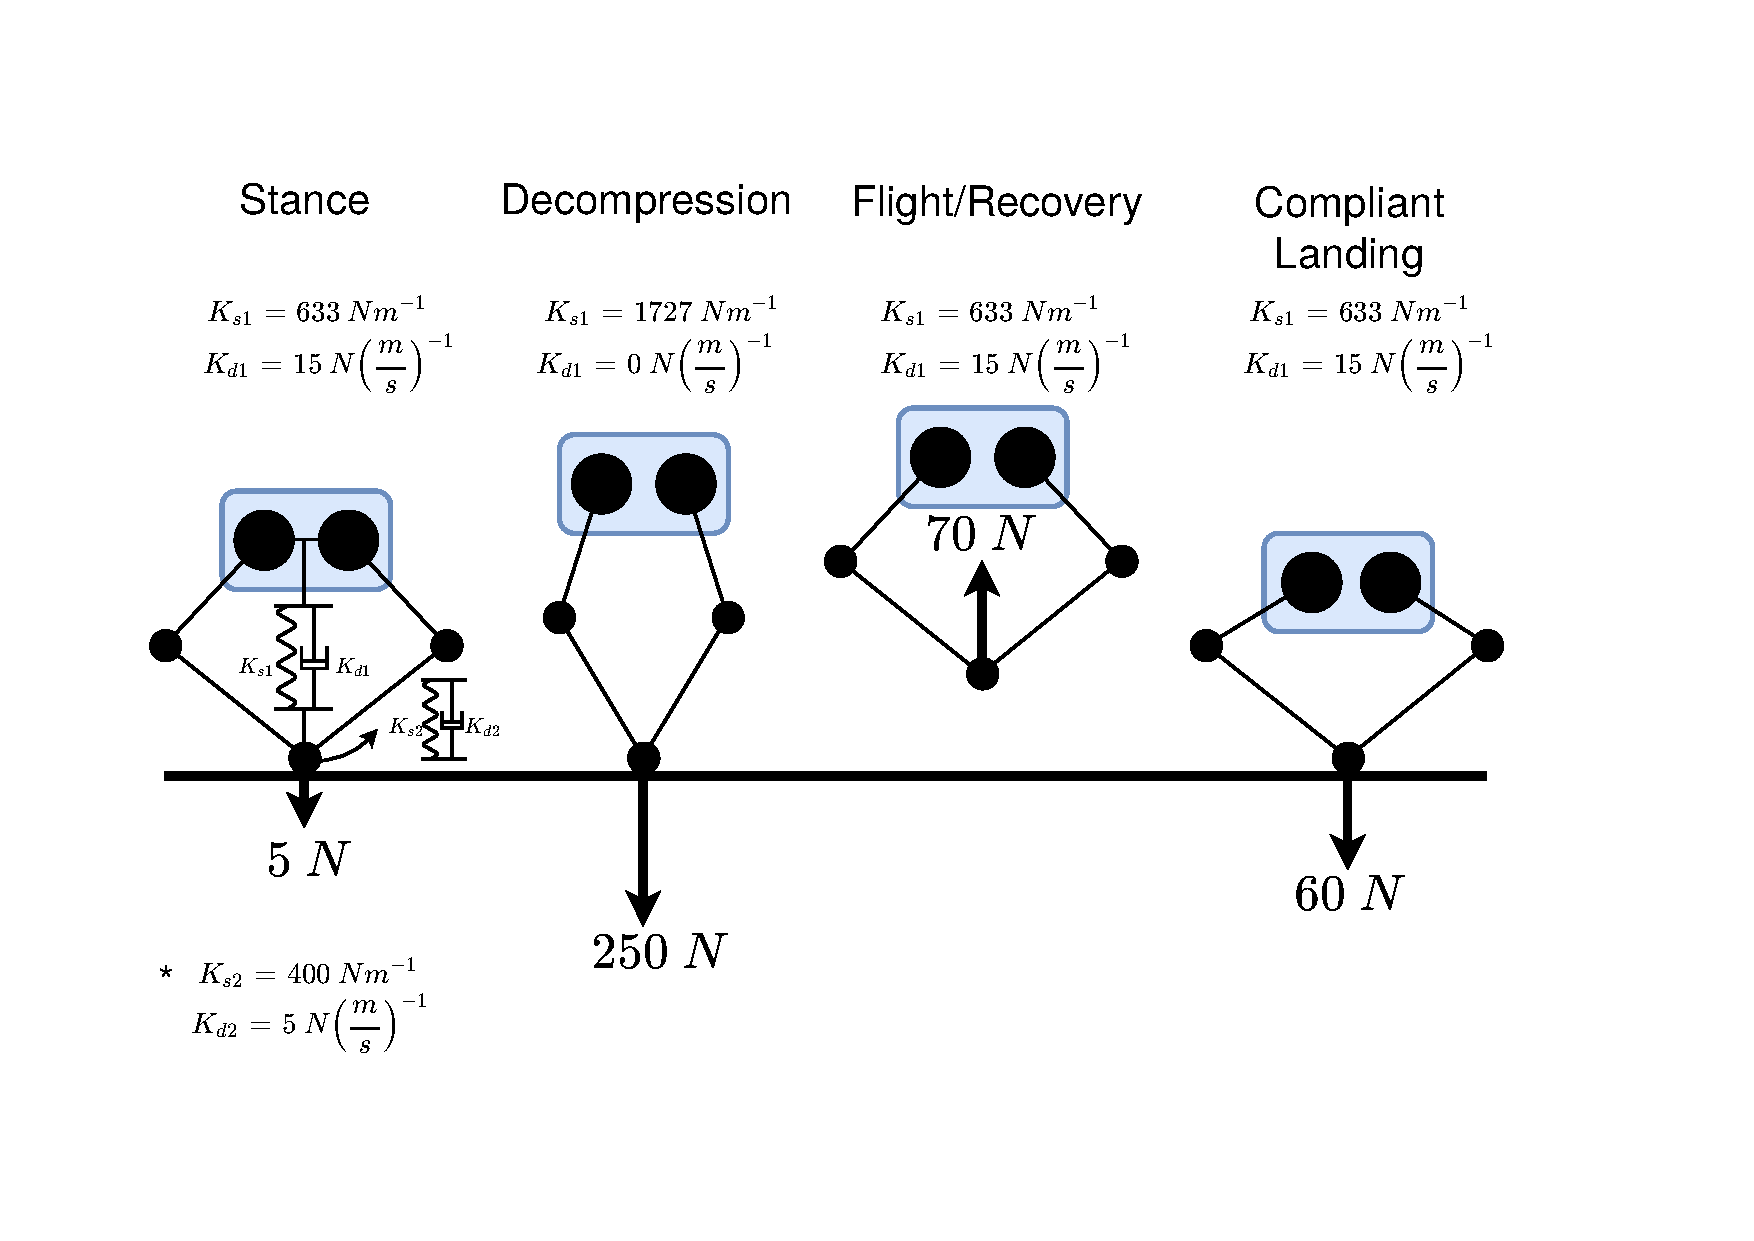
\includegraphics[clip, trim = 2.5cm 2cm 4cm 2cm, width=1\textwidth]{images/experiments/jump/jump-phases.pdf} 
\caption{Jump phases and experimental setup.}
\label{fig:jump-phases-experiment}
\end{figure}

\subsection{Configuration of Jump Phase Parameters}

Spring-damper mass motion of the leg model was theoretically developed in \cref{sec:Spring-damper Mass Motion}. Ideal spring-damper constants for flight, impact and launch were developed using conservation of energy relationships and spring-damper dynamic equations. 

The table of spring-damper constants and other configuration parameters, \cref{tbl:Leg launch virtual model configuration}, was found for ideal jump phase dynamics relating to the spring constants in \cref{fig:Leg spring-damper virtual model}. 

Parameters were derived both experimentally and theoretically. The theoretical (orange), drop test experimental (blue), and spring-damper test experimental (red) configuration parameters were highlighted appropriately.

\begin{table}[]
\centering
\begin{tabular}{llllll}
\textbf{Phase}       & \textbf{$K_{s1}\ [Nm]$}                 & \textbf{$K_{d1}\ [N/(m/s)]$}       & \textbf{$K_{s2}\ [N/m]$}     & \textbf{$K_{d2}\ [N/(m/s)]$} & \textbf{$r\ [m]$}                    \\
Stance               & 632.8                                   & \cellcolor[HTML]{00D2CB}15         & \cellcolor[HTML]{00D2CB}400 & \cellcolor[HTML]{00D2CB}5    & 0.25                                 \\
Decompression launch & \cellcolor[HTML]{FFC702}\textbf{1726.6} & \cellcolor[HTML]{FFC702}\textbf{0} & \cellcolor[HTML]{00D2CB}400 & \cellcolor[HTML]{00D2CB}5    & \cellcolor[HTML]{FFC702}\textbf{0.4} \\
Recovery             & \cellcolor[HTML]{FD6864}632.8           & \cellcolor[HTML]{00D2CB}15         & \cellcolor[HTML]{00D2CB}400 & \cellcolor[HTML]{00D2CB}5    & \cellcolor[HTML]{FD6864}0.3          \\
Compliant landing    & \cellcolor[HTML]{FFC702}\textbf{632.8}  & \cellcolor[HTML]{00D2CB}15         & \cellcolor[HTML]{00D2CB}400 & \cellcolor[HTML]{00D2CB}5    & \cellcolor[HTML]{FFC702}\textbf{0.3}
\end{tabular}
\caption{Leg launch virtual model configuration.}
\label{tbl:Leg launch virtual model configuration}
\end{table}

\subsection{Finite State Machine and Triggering}

\Cref{listing:Jump control condition loop} in \cref{app:Jump Experiment} shows the code implementation of a finite state machine that determines which spring-damper parameters are used in which phase of jumping. A similar finite state machine virtual model control method was considered in \cite{Pratt2001} for phase changes.

Using \textit{if statements} various conditions were tested to determine the phase of jumping. Leg radial distance, foot force and time were used as conditions for phase change points. 

Theoretically a more reliable method for determining ground contact would have been to use a foot trigger or a distance sensor. Both of these methods were attempted, but when it came to testing neither were reliable. The foot trigger was subjected to multiple impacts and was not mechanically robust. Due to the long cable from the foot trigger to the microcontroller, and possibly the noise from motor EMI, caused the foot trigger to be triggered prematurely causing damaging mid-air high gain force commands. The distance sensor beam width was too wide and due to the construction of the platform did not reliably detect the distance of the body from the platform. 

The most reliable method proved to be using the radial set-point to determine when the leg was compressed after impact. 

\subsection{Testing Platform Setup}

The testing platform designed in \cref{subsec:Testing Platform} was used during the jump experiments. It was securely mounted against a vertical backdrop to ensure it was steady during jumps. During tuning of the leg prior to jumps it was secured on the linear guide before being allowed to freely rest on the base. The sandpaper and rubber foot ensured the foot did not slip before launching and during impact.

\subsection{Video Data Extraction}

In \cref{app:Jump Experiment} the data extracted from the video relating to body height, velocity, and phase versus time is included to show the data used to plot \cref{fig:height-time-jump,fig:velocity-time-jump,fig:acc-time-jump}. 

The video was filmed at $24\ fps$. The testing platform linear guide has markers on it indicating height. For each frame the relevant height data, measured from the original resting height of the leg, was recorded along with the time. Using the backwards difference the velocity and acceleration for the interval was calculated - as such the values must be critically analysed.

\subsection{Experimental Limitations}

The jump experiment was limited by the motor driver limit of $60\ A$. Foot force is related to motor current - to achieved height control or accurate foot force impulses a larger current limit is needed. During experimentation the current saturated immediately during jumping, showing that a larger current range was needed. 

When two consecutive high energy jumps were attempted a motor driver current cut-out was triggered. A video extract of this action can be seen in \cref{app:Jump Experiment} \cref{fig:Motor driver over-current cut-out}. 

To perform multiple consecutive jumps as seen in \cref{sec:Consecutive Jump Repeatability}, a lower energy jump was performed with a maximum jump height of $0.25\ m$.

\subsection{Data Analysis}

\subsubsection{Launch Phase}

In order to achieve as rapid a vertical acceleration as possible the motor current needs to be saturated. \Cref{fig:jump-motor-current-feedback} shows that as the launch phase starts the current command is saturated at just under the motor driver peak current of $60\ A$ to avoid current cut-out.

The radial foot force of \cref{fig:Jump foot force output} is directly related to the difference between the radial set-point, summarised in \cref{tbl:Leg launch virtual model configuration}, and the actual leg radius feedback. The foot force instantaneously increased from a magnitude of near $0\ N$ to a maximum of $-270\ N$ - in reality the foot force during this transition may be more slow to react, as the foot force is theoretically determined using the virtual model.

The launch phase has a duration of $10\ ms$ before the next control phase takes over. As the leg radius extends beyond $0.38\ m$ the next phase, the flight phase, is triggered as expected. 

\subsubsection{Flight Phase}

At this point the current command switches polarity quickly to restore the leg position for landing. The leg radius is restored within $15\ ms$ to the radial set-point of $0.3\ m$ with no overshoot or steady state error. This validates the control method and virtual model parameters for the flight phase. In three sample periods the controller managed to accurately command a kinematic set-point.

During the free-fall phase the downwards acceleration of the body had a mean value of $9.51\ m/s^2$ as seen in \cref{fig:acc-time-jump}. This is expected, with a gravitational constant of $9.81\ m/s$ and a coefficient of kinetic friction as calculated in \cref{sec:Mechanical Impedance}, the mean body acceleration should be less than that of gravity.

The impact phase occurs approximately $20\ ms$ later leaving lots of room for error in leg restoration. 

\subsubsection{Landing Phase}

During the landing phase the radial length of the leg decreased to a minimum of approximately $0.24\ m$, as seen in \cref{fig:Jump foot radial position and velocity}. This was a relatively severe undershoot, with a set-point of $0.3\ m$. The radius recovered to $0.28\ m$ within $15\ ms$ or three sample points. This shows that during impact a lot of force is experienced. The spring-damper constants should be increased in future to account for this. The impact was absorbed without oscillation, and so was still stable as designed.

\Cref{fig:jump-motor-current-feedback} shows the current feedback versus time. The current was very oscillatory. Increasing the control sampling frequency would have dealt with the high speed impact with more accuracy and perhaps have prevented the radial undershoot. 

Although the foot force during impact was relatively small compared to the launch phase, the current was at near it's maximum upon impact. This shows the effect of saturation. At launch, the leg wanted to output $-270\ N$ of force, and would have done so without the current saturation, but in practise it probably experienced a much lower foot force. If a foot force plate was available for measurement, the true foot force could have been determined.

\subsubsection{Foot Placement}

In the plot of radial and angular foot force versus time in \cref{fig:Jump foot force output}, it can be clearly seen that the angular force makes up very little of the total foot force. This shows that the control system is accurately keeping the foot at a zero angular set-point and that the launch and landing phases put very little stress in the angular direction. 

\Cref{fig:Jump Freefall Impact and Compliant Landing Phase} confirms the accurate angular foot placement where extracted video frames show minimal angular movement, with the linear guide as a reference point. Even during transitions between phases, where the most angular movement is expected, very little was experienced.

\subsubsection{Jump Energy}

The theoretical jump energy can be calculated using \cref{eq:experimental-jump-energy}. 

\begin{equation} \label{eq:experimental-jump-energy}
E_{jump} = mgh_{max}\times \frac{1}{Efficiency[\%]}
\end{equation}

Assuming the jump is $100\ \%$ efficient and the maximum jump height logged of $0.4$ is used, the jump energy is $8.63\ J$. This jump energy is compared to other similar legged robots in \cref{tbl:Robot performance comparison}.

\subsubsection{Control Sampling Time}

The controller performed well considering that many of the critical sections of the jump phases occurred in under $20\ ms$ or 4 sample periods. A higher sampling frequency, in the $kHz$ time-scale would result in a much higher fidelity virtual model, but in practise the sampling frequency of $200\ Hz$ worked well both for jump experimentation and the spring-damper tests of \cref{sec:Virtual Spring-damper Tests}.

\subsection{Summary}

Based on the experimental data analysis, the following conclusions can be made:
\begin{enumerate}
\item The motor driver peak current limit of $60\ A$ severely limits the amount of force available during launching. Theoretically a $-270\ N$ force would have been experienced with a current saturation of around $150\ A$, but in practise it was much lower and limited how much control could be had over impulse forces and how high the leg could jump.
\item At a $200\ Hz$ sampling rate, once again limited by the motor driver response time, high fidelity virtual model control is difficult to achieve. In practise many of the critical phase sections were less than $20\ ms$, leaving 4 sample points for the controller to effect the necessary commands.
\item The foot placement during launch and recovery was accurate and well controlled. During impact a higher spring constant and damping were required to achieve less undershoot, but no oscillation was experienced.
\item Considering the current limit of $60\ A$, the energy delivered, $8.63\ J$, compared favourably to the GOAT leg, $20.11\ J$ with three motors, a higher current limit, and custom controllers and gearing.
\end{enumerate}

\begin{figure}
\centering
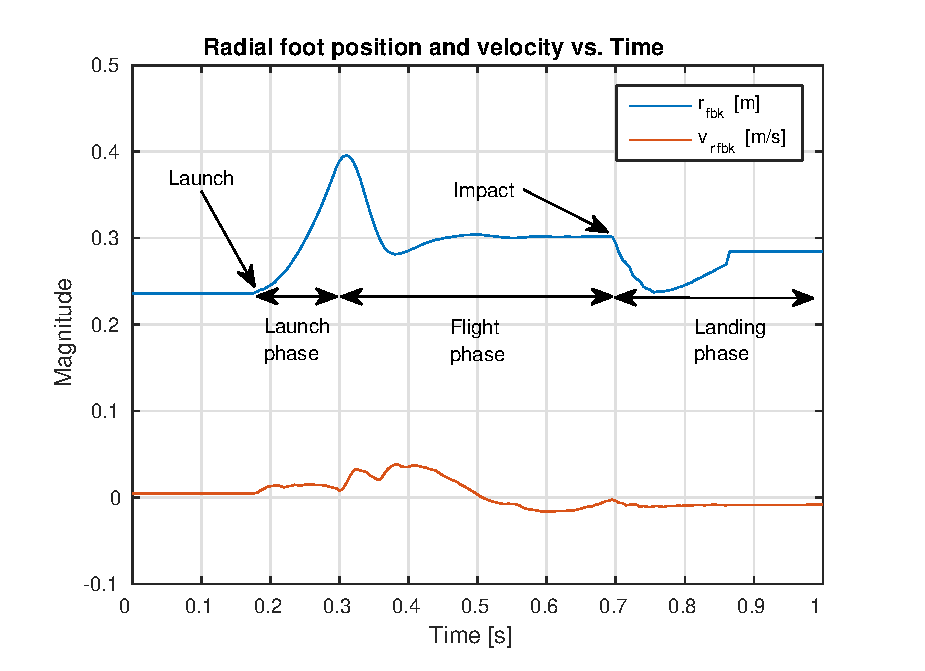
\includegraphics[width=0.9\textwidth]{images/experiments/jump/jump-foot-position-velocity.eps} 
\caption{Jump foot radial position and velocity (launch and compliant landing).}
\label{fig:Jump foot radial position and velocity}
\end{figure}

\begin{figure}
\centering
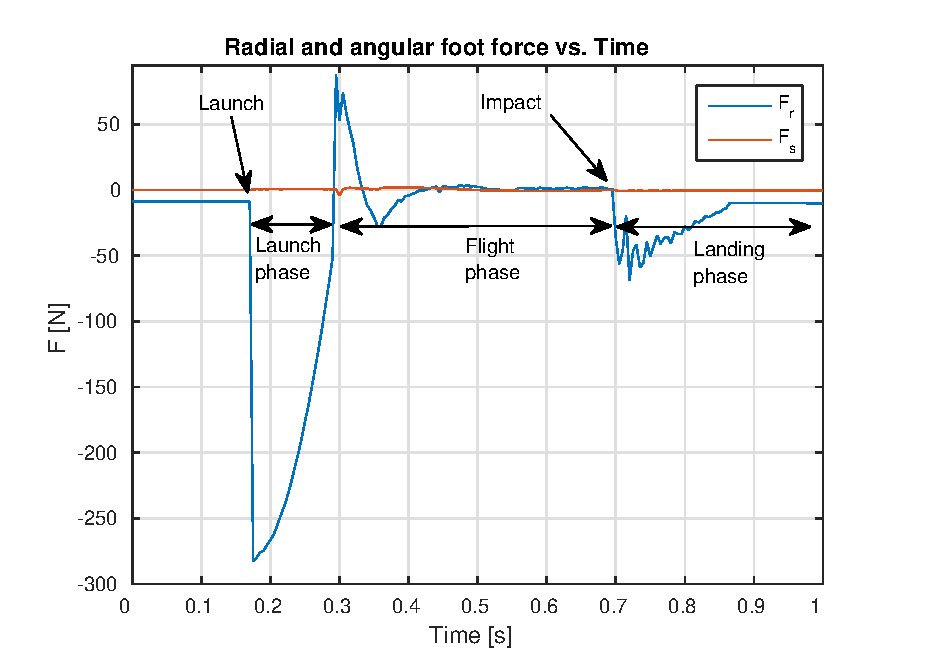
\includegraphics[width=0.9\textwidth]{images/experiments/jump/jump-foot-force.eps} 
\caption{Jump foot force output (launch and compliant landing).}
\label{fig:Jump foot force output}
\end{figure}

\begin{figure}
\centering
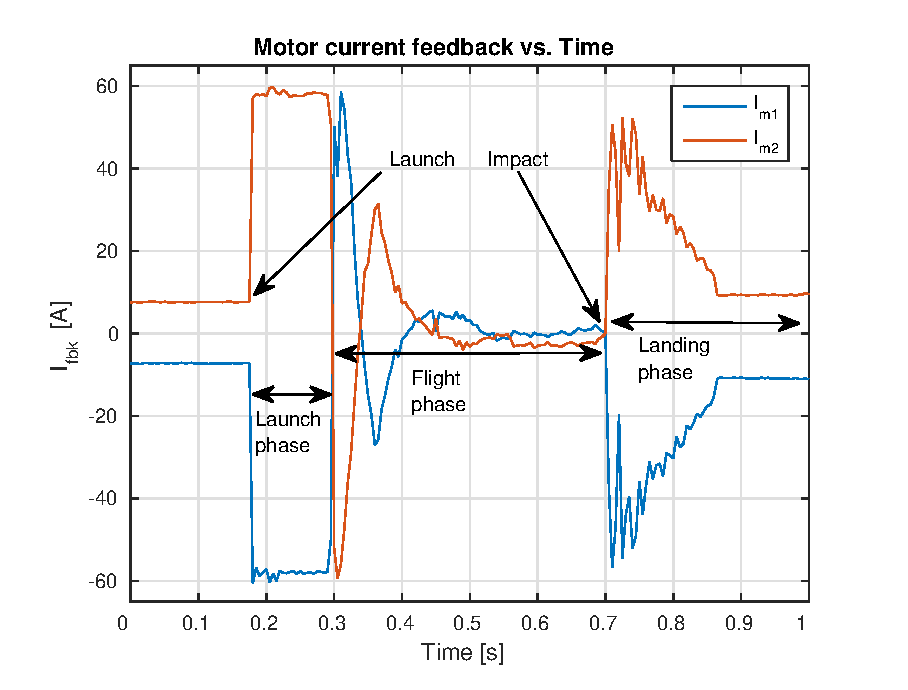
\includegraphics[width=0.9\textwidth]{images/experiments/jump/jump-current-feedback.eps} 
\caption{Jump motor current feedback (launch and compliant landing).}
\label{fig:jump-motor-current-feedback}
\end{figure}

\begin{figure}
\centering
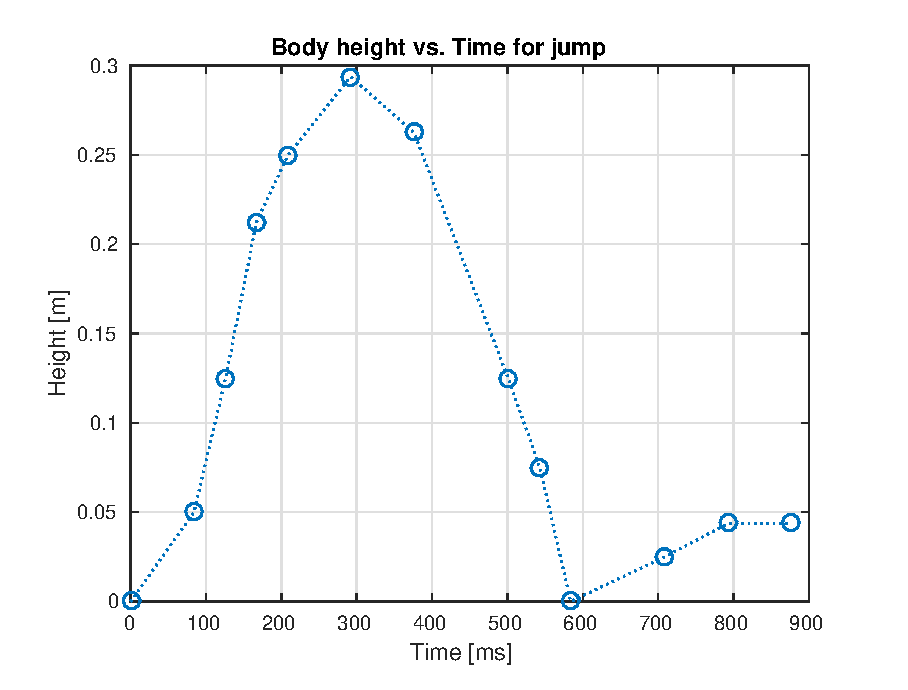
\includegraphics[width=0.9\textwidth]{images/experiments/jump/height-vs-time.eps} 
\caption{Height vs. time plot relative to body starting position.}
\label{fig:height-time-jump}
\end{figure}

\begin{figure}
\centering
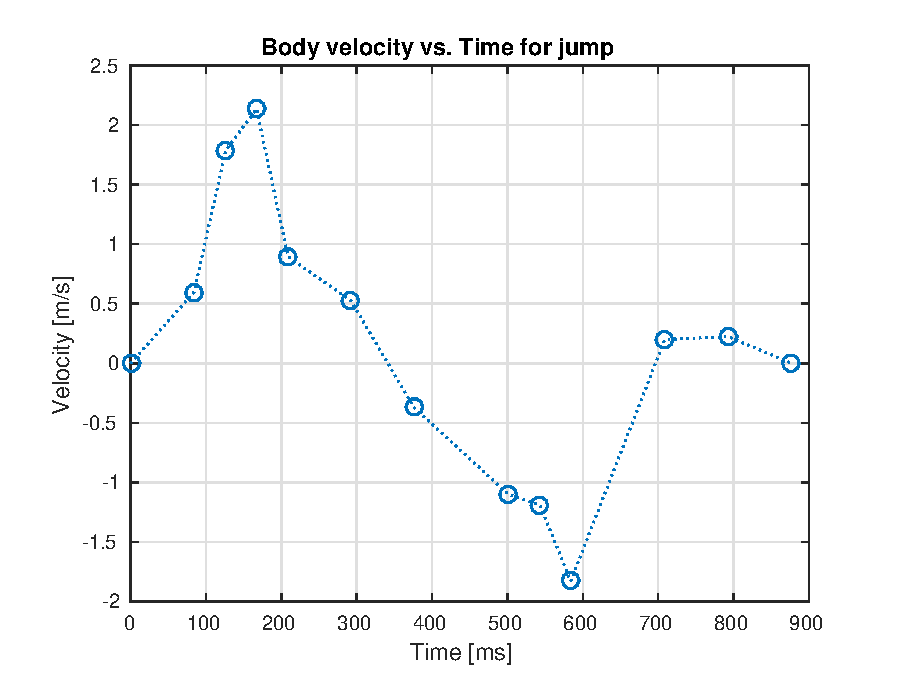
\includegraphics[width=0.9\textwidth]{images/experiments/jump/velocity-vs-time.eps} 
\caption{Velocity vs. time plot relative to body starting position.}
\label{fig:velocity-time-jump}
\end{figure}

\begin{figure}
\centering
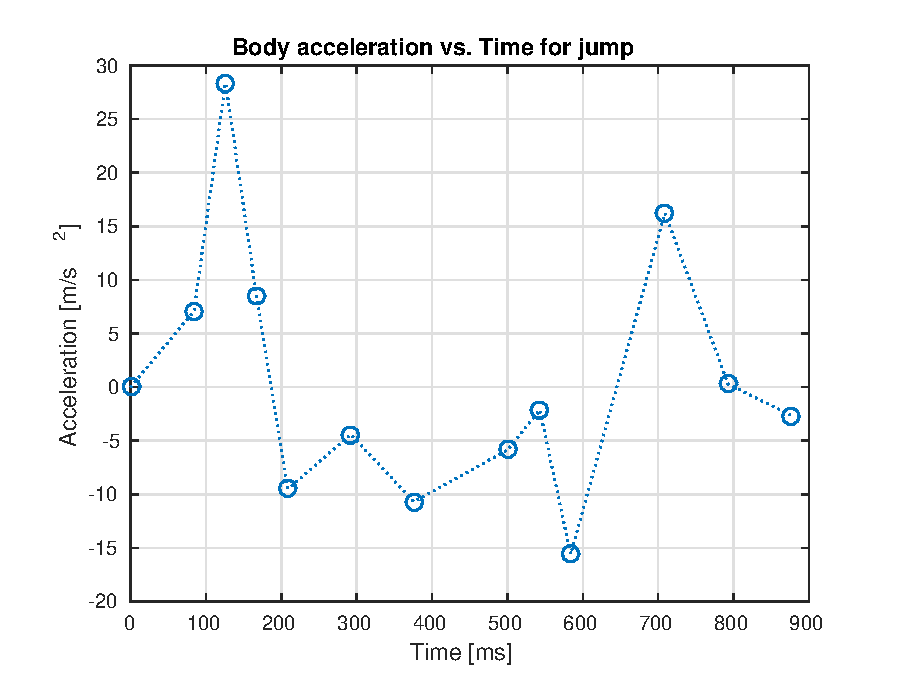
\includegraphics[width=0.9\textwidth]{images/experiments/jump/acceleration-vs-time.eps} 
\caption{Acceleration vs. time plot relative to body starting position.}
\label{fig:acc-time-jump}
\end{figure}

\begin{figure}
\centering
\subfloat[][Frame 0: Stance.]{
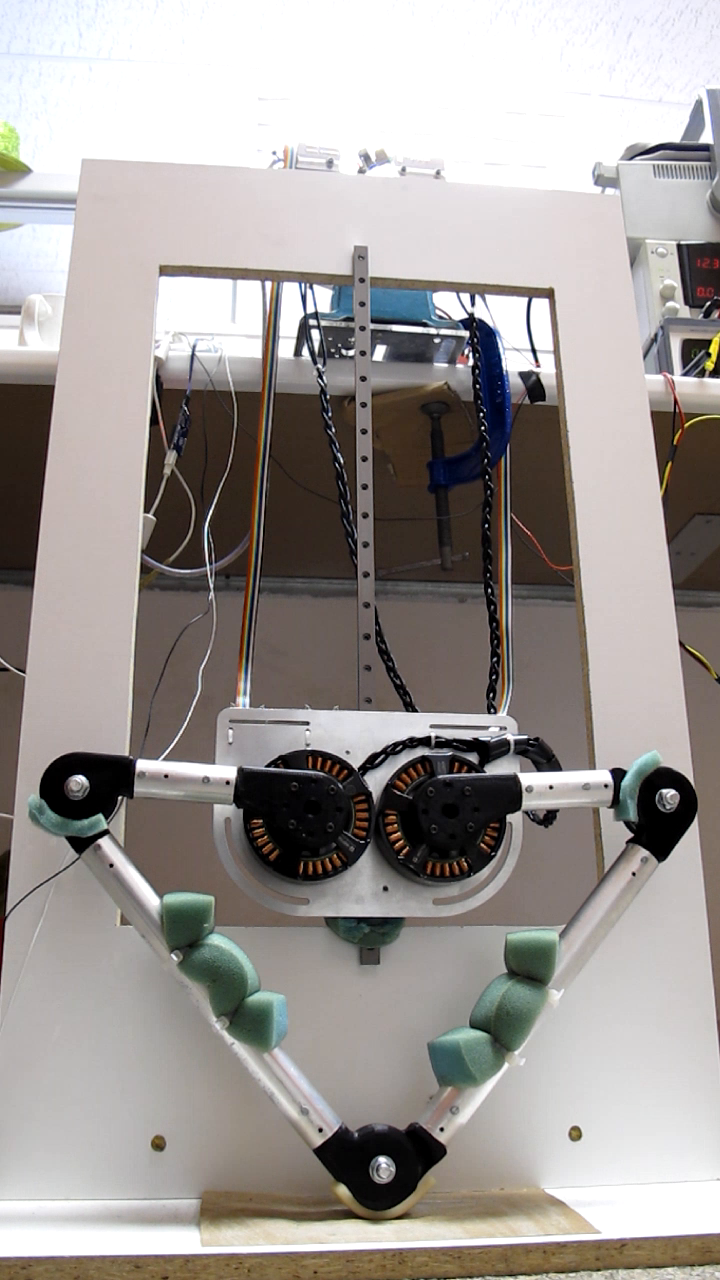
\includegraphics[width=0.3\textwidth]{images/experiments/jump/0.png} 
}
~
\subfloat[][Frame 1: Decompression.]{
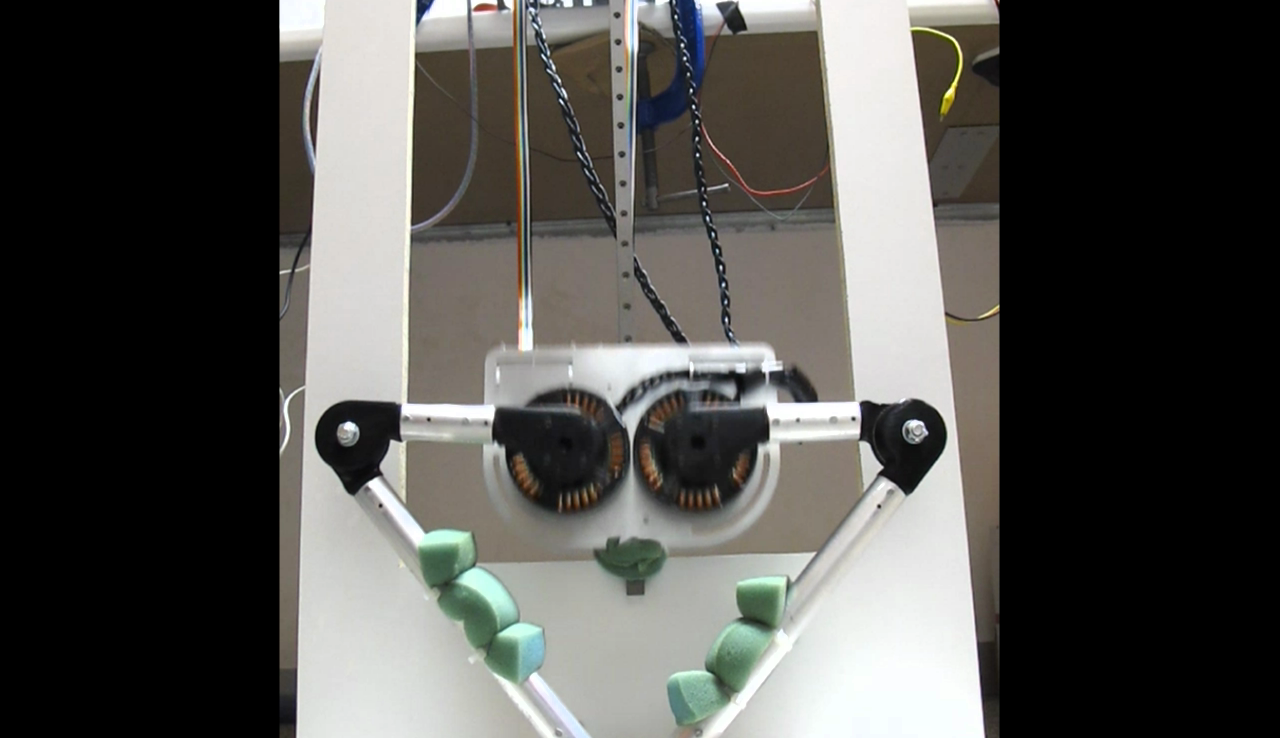
\includegraphics[width=0.3\textwidth]{images/experiments/jump/1.png} 
}
~
\subfloat[][Frame 2: Decompression.]{
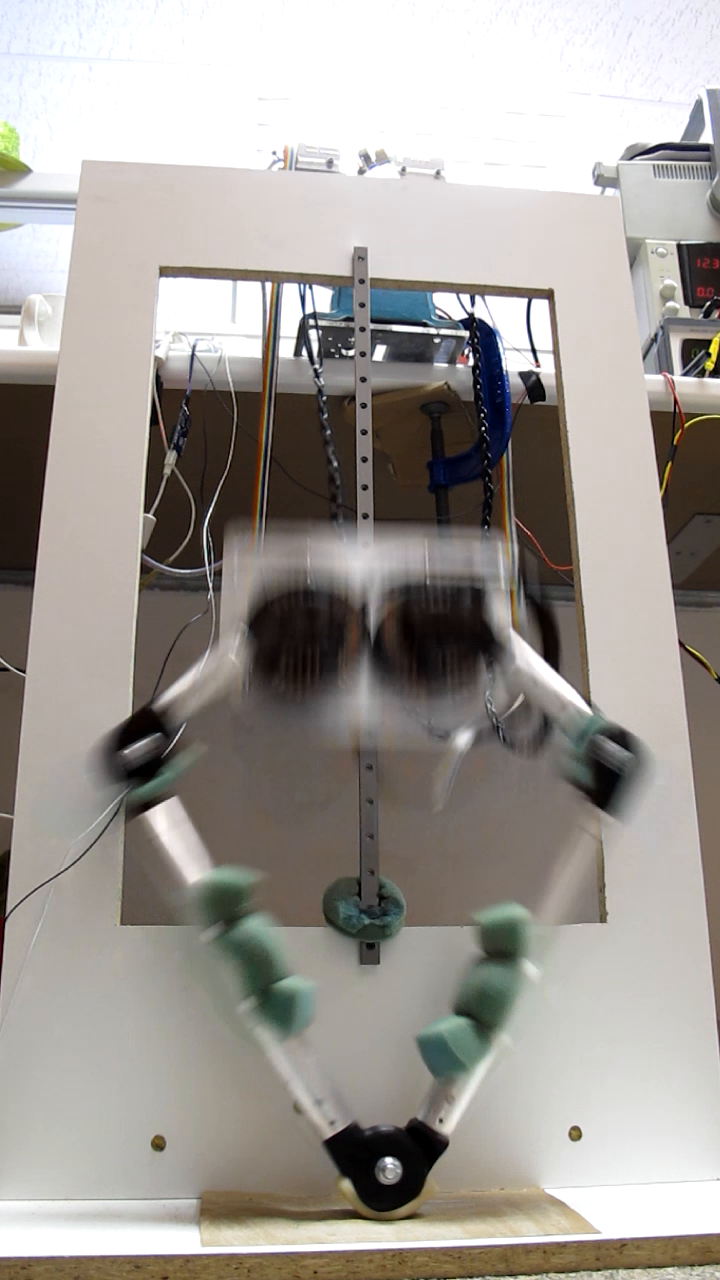
\includegraphics[width=0.3\textwidth]{images/experiments/jump/2.png} 
}

\subfloat[][Frame 3: Flight.]{
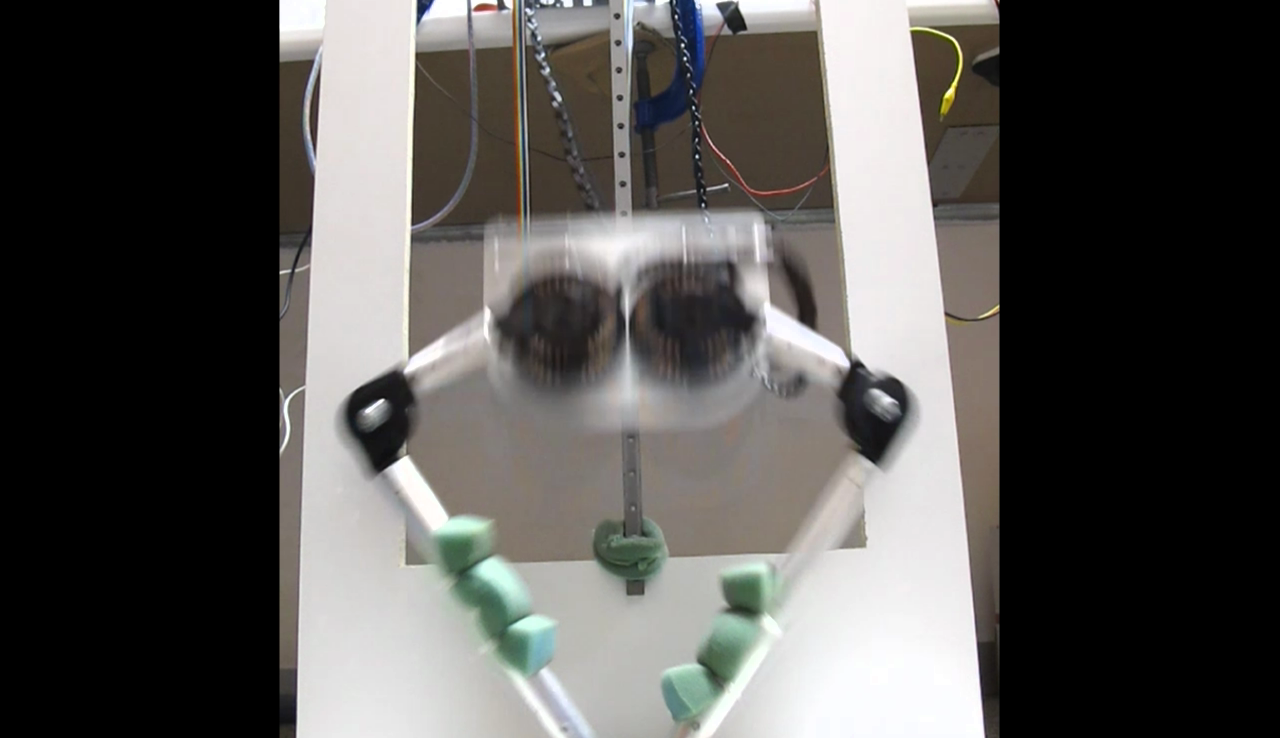
\includegraphics[width=0.3\textwidth]{images/experiments/jump/3.png} 
}
~
\subfloat[][Frame 4: Flight/recovery.]{
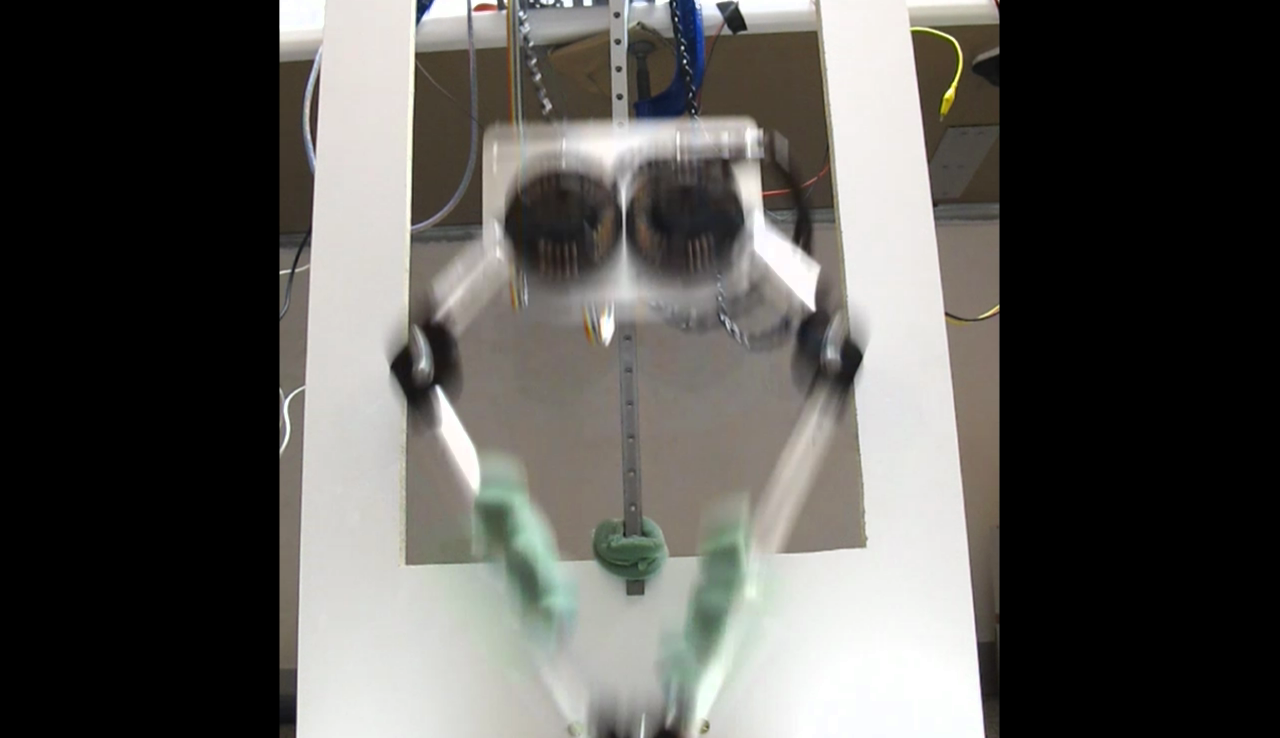
\includegraphics[width=0.3\textwidth]{images/experiments/jump/4.png} 
}
~
\subfloat[][Frame 5: Flight/recovery.]{
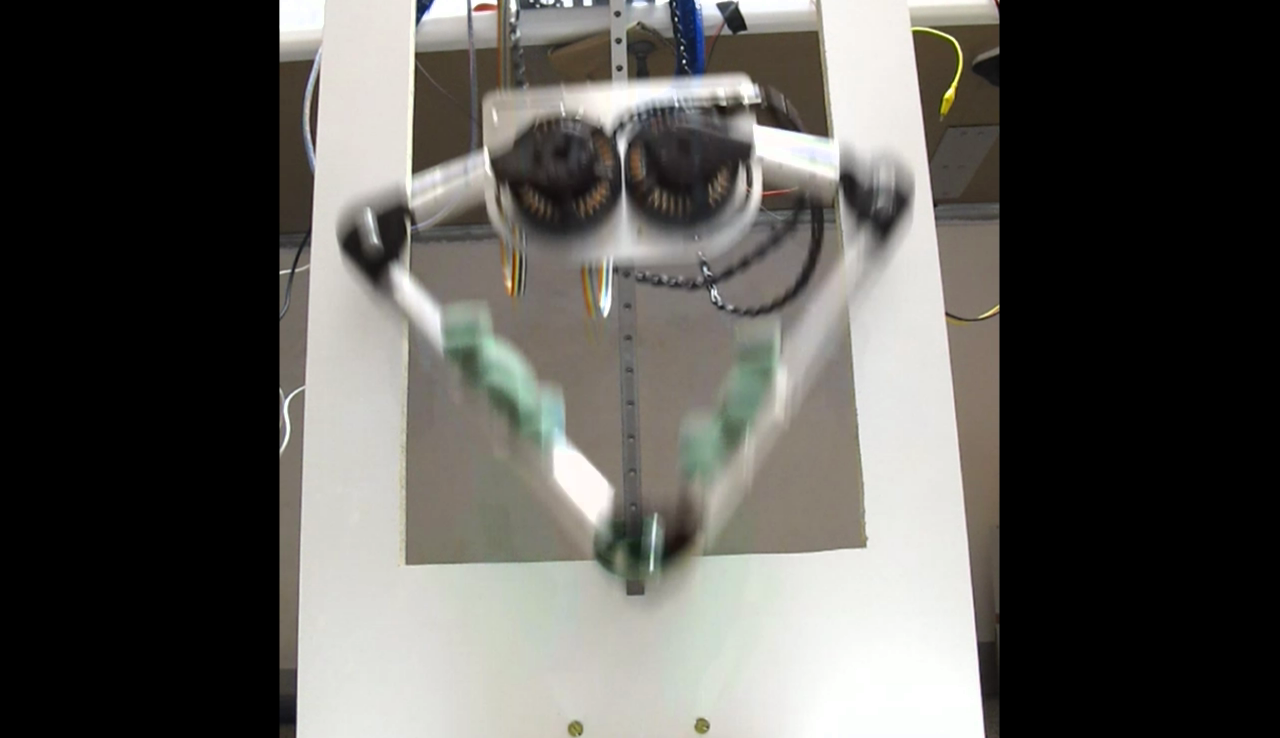
\includegraphics[width=0.3\textwidth]{images/experiments/jump/5.png} 
}
\caption{Jump: Stance and Flight Phase.}
\label{fig:Jump Stance and Flight Phase}
\end{figure}

\begin{figure}
\centering
\subfloat[][Frame 6: Freefall.]{
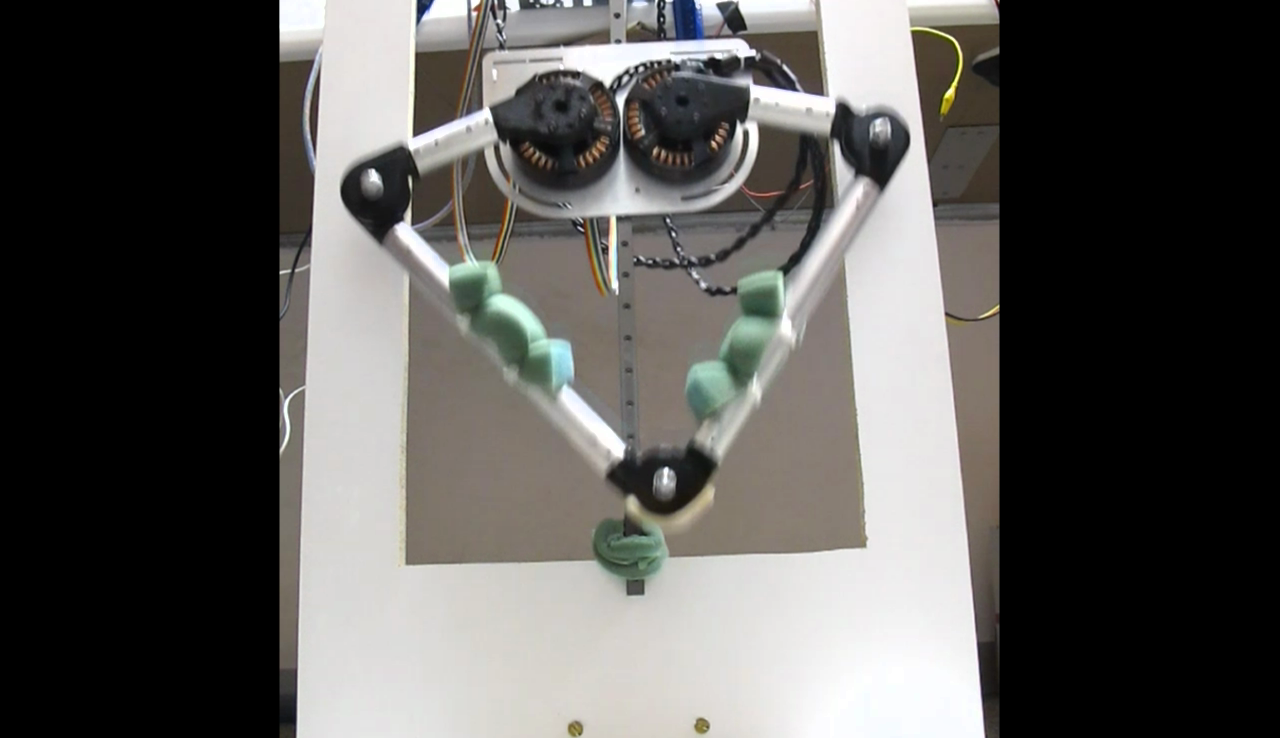
\includegraphics[width=0.3\textwidth]{images/experiments/jump/6.png} 
}
~
\subfloat[][Frame 7: Freefall.]{
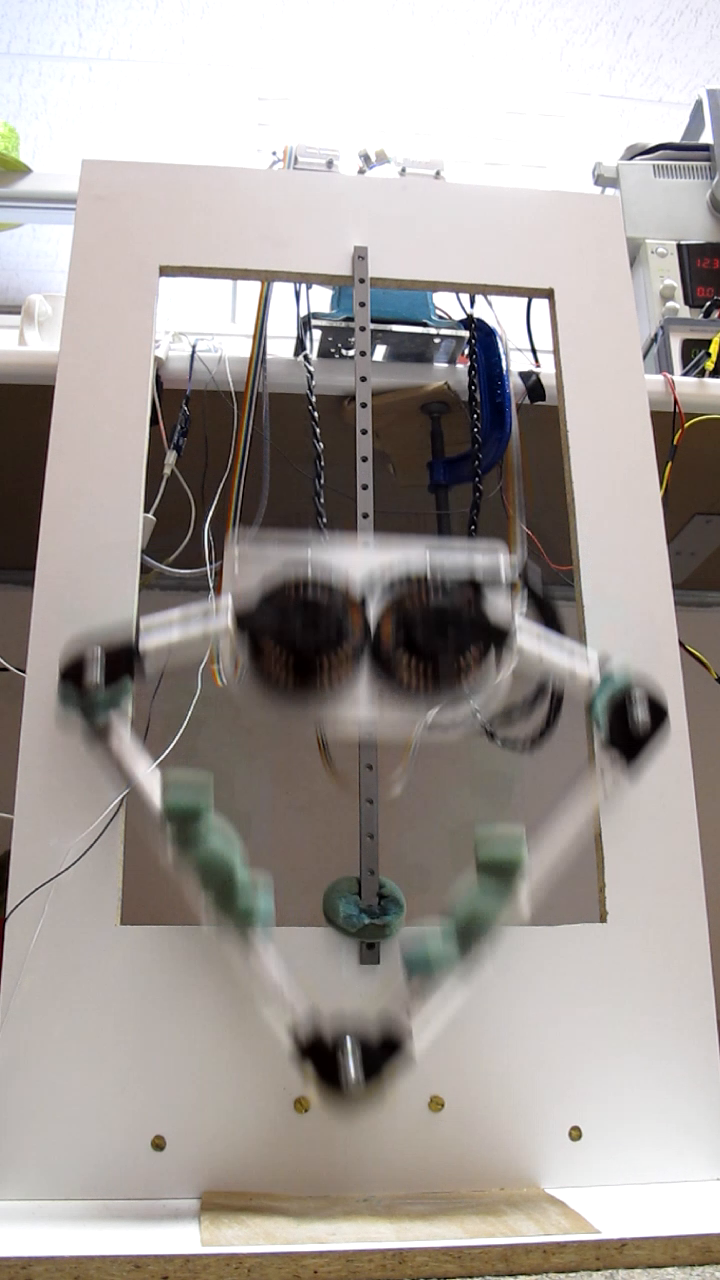
\includegraphics[width=0.3\textwidth]{images/experiments/jump/7.png} 
}
~
\subfloat[][Frame 8: Impact.]{
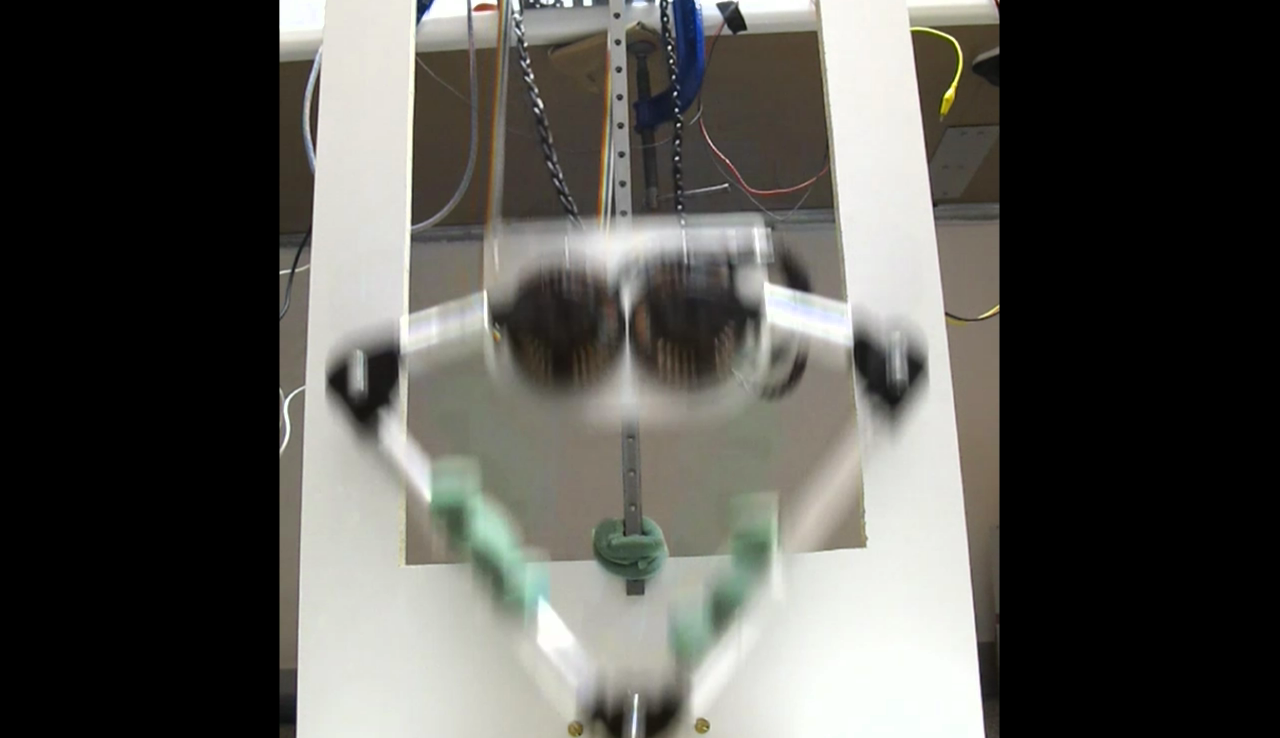
\includegraphics[width=0.3\textwidth]{images/experiments/jump/8.png} 
}

\subfloat[][Frame 9: Compliant landing.]{
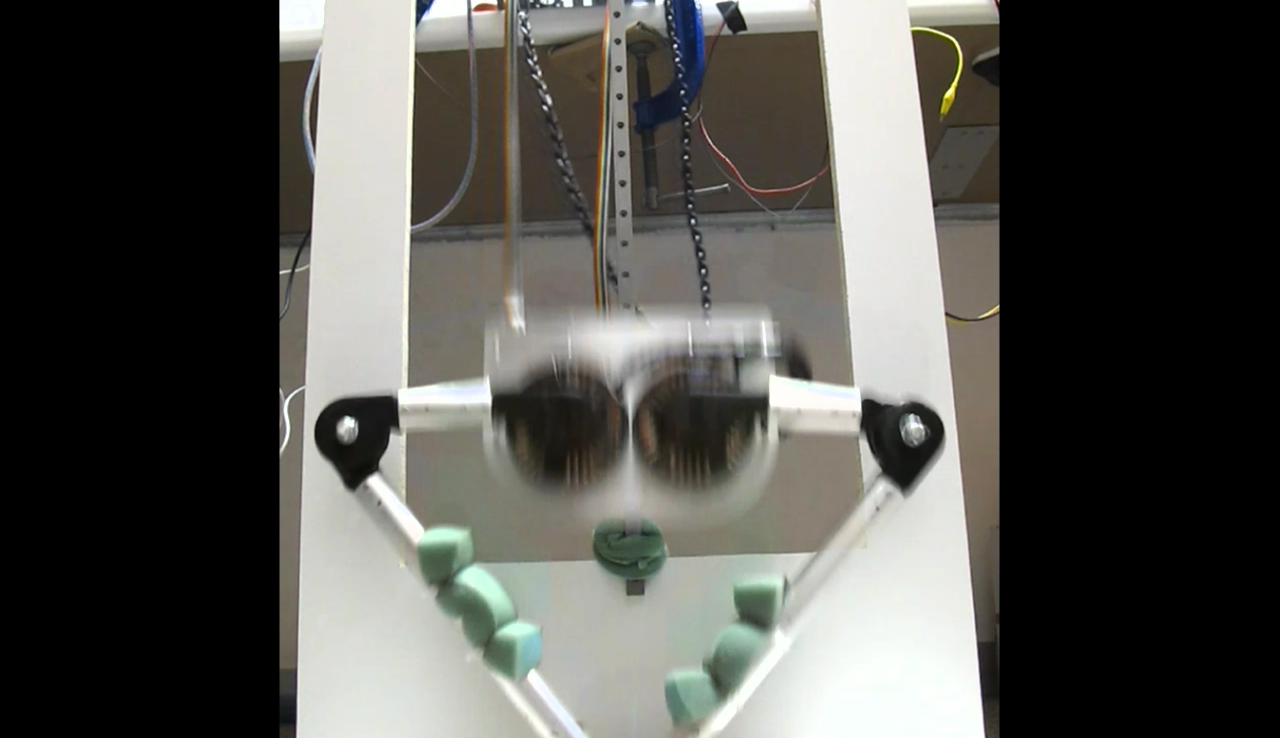
\includegraphics[width=0.3\textwidth]{images/experiments/jump/9.png} 
}
~
\subfloat[][Frame 10: Compliant landing.]{
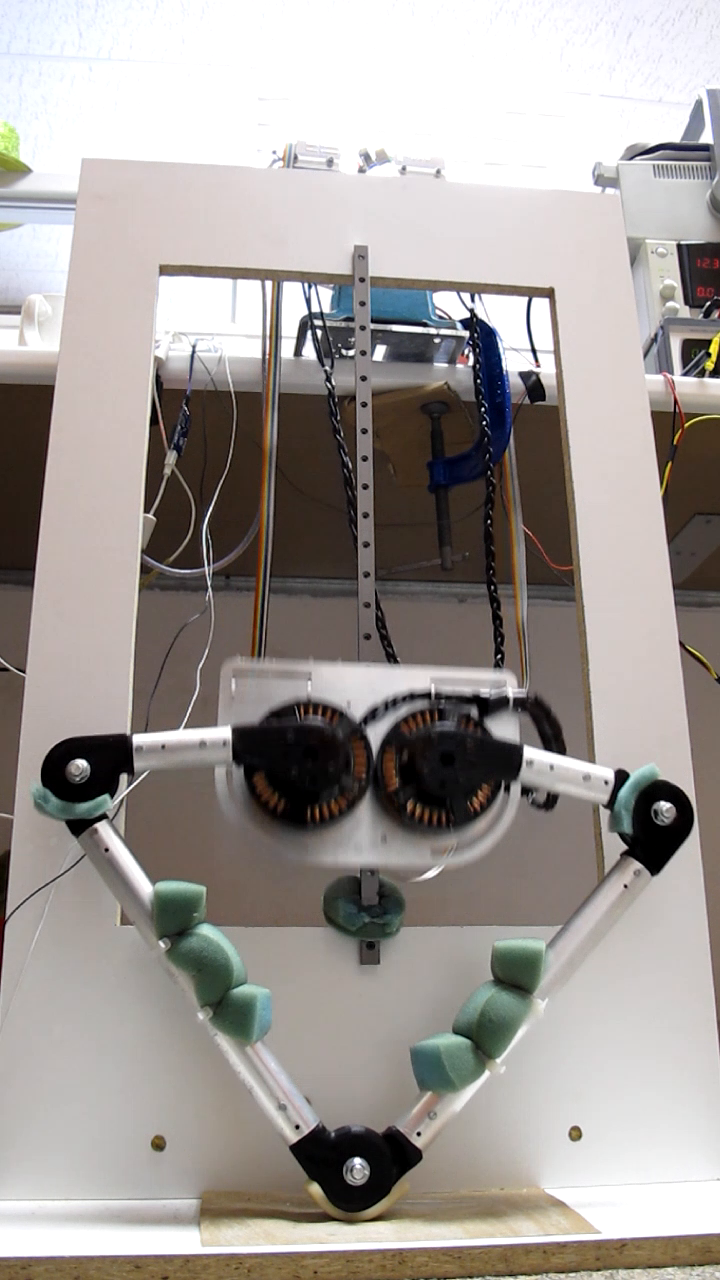
\includegraphics[width=0.3\textwidth]{images/experiments/jump/10.png} 
}
~
\subfloat[][Frame 11: Compliant landing.]{
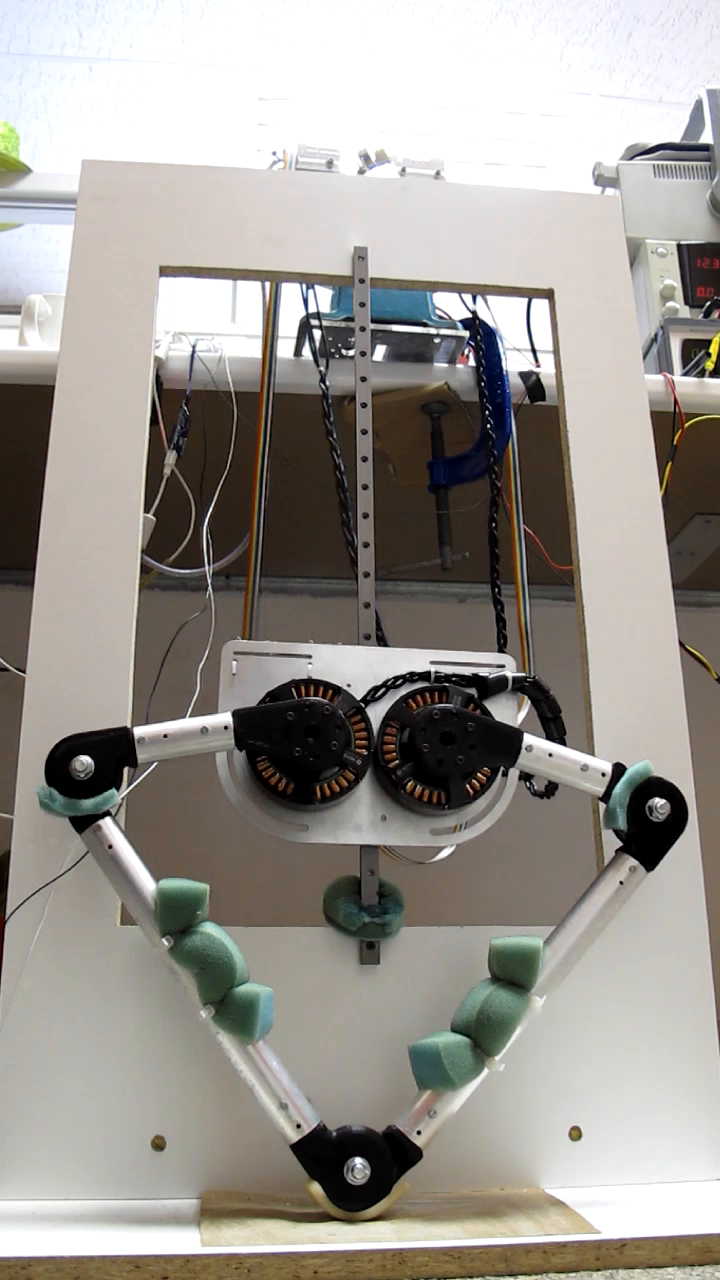
\includegraphics[width=0.3\textwidth]{images/experiments/jump/11.png} 
}
\caption{Jump: Freefall, Impact and Compliant Landing Phase.}
\label{fig:Jump Freefall Impact and Compliant Landing Phase}
\end{figure}

\section{Consecutive Jump Repeatability}
\label{sec:Consecutive Jump Repeatability}

In order to test the platform's design with robustness and repeatability as performance measures, multiple consecutive jump were performed without interfering with the control system or platform in any way.  

The leg was mounted on the platform in a central foot position before the launch sequence was initialised. Seven consecutive jumps were performed to a moderate height of $25\ cm$. 

A plot of foot force versus time was created with all seven plots overlayed on the same set of axis, as seen in \cref{fig:multi-jump-plot}. The starting points of the jumps were synchronised to show changes in jump patterns. 

\subsection{Data Analysis}

A maximum foot force deviation of $32\ N$ was seen for jump 4 with the mean being a foot force of $130\ N$. 

A maximum time phase shift of $0.15\ s$ was seen between jumps, over a total mean jump duration $0.7\ s$ - so the time deviation was a $21\ \%$ change. 

The foot forces all settled at approximately the same value of $8\ N$ before dropping to $-10\ N$ in preparation for the next jump. This pattern was consistent.

Both of the above deviation measurements were thrown off by the outlier of jump 4. If this jump is ignored due to experimental error, then the maximum deviation in time is approximately $0.06\ s$, or $8.57\%$, and for force is negligible.

\subsection{Summary}

The experimental data analysis showed two results:
\begin{enumerate}
\item The leg control system is capable of \textbf{robust} force control with a \textbf{negligible deviation} for force and time.
\item The construction and design of the robotic leg platform enables \textbf{reliable and repeatable force control} to implement consecutive jumping sequences.
\end{enumerate}

\begin{figure}
\centering
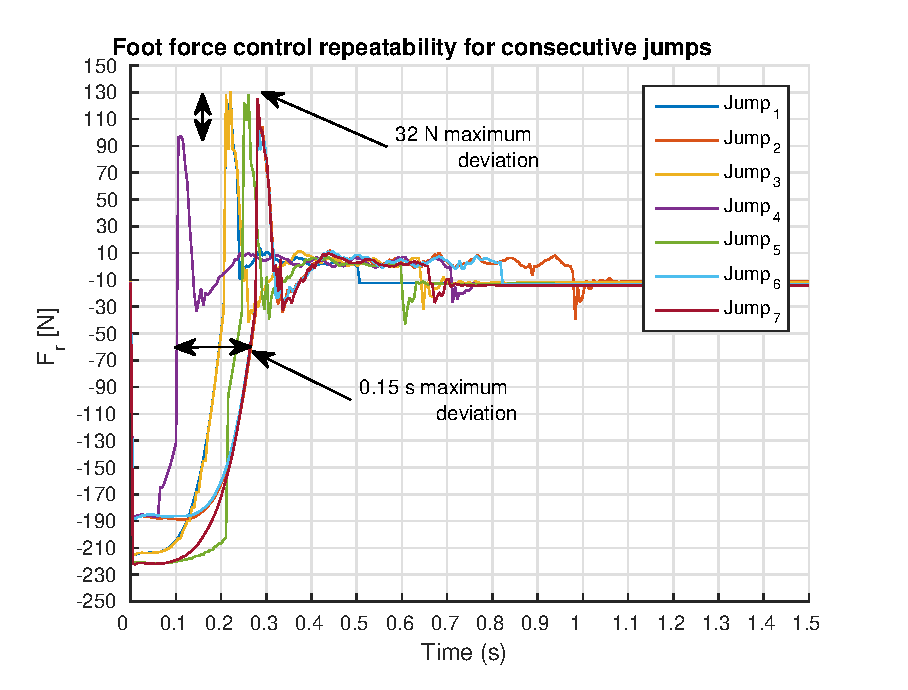
\includegraphics[width=1\textwidth]{images/experiments/multi-jump-plot.eps} 
\caption{Consecutive jump foot force to investigate repeatability.}
\label{fig:multi-jump-plot}
\end{figure}

\section{Current Tracking}

For high fidelity force control using a virtual model to be achieved, two things need to be ensured:
\begin{enumerate}
\item Transparent and efficient torque coupling between motor and linkages.
\item Accurate high speed current tracking during dynamic movements. 
\end{enumerate}

The transparency and efficiency of the torque coupling is almost entirely a mechanical specification. By using a direct drive motor system this is mostly taken care of.

Accurate high speed current tracking ensures that when an impact occurs, the foot force will respond appropriately and absorb the impact energy (assuming a spring-damper virtual model). 

\subsection{Data Analysis}

\Cref{fig:Current control tracking} shows a plot of current feedback from motor driver 1 versus the current command from the force controller - during an impact after the jump test in \cref{sec:Jump Test}. The force command is ideally directly related to the torque constant, $K_t$, and Jacobian force mapping derived in \cref{sec:Force Control}. 

In \cref{fig:Current control tracking} at the point of impact, the current command leads the current feedback in a sudden negative drop. The current feedback tracks the command very well with the expected one sample delay. In reality, the current tracking may be better than we are able to measure - if the current could be measured directly after the command this would give a better idea of the true performance. 

During the recovery period from $0.1\ s$ to $0.2\ s$ the set-point tracking is consistent and stable. After the current command settles we can see that there is zero steady state error.

\subsection{Summary}

The current \textbf{reacts quickly} to sudden high magnitude changes. Set-point tracking is at most \textbf{delayed by one-sample}, $5\ ms$, and \textbf{tracks consistently}. \textbf{No error} exists during steady state. 

\begin{figure}
\centering
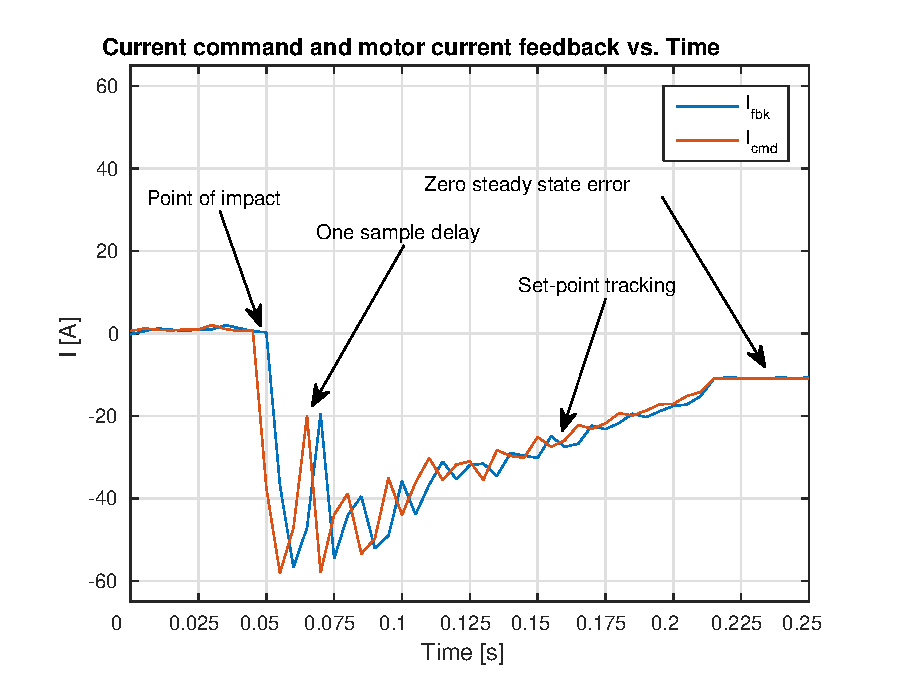
\includegraphics[width=1\textwidth]{images/experiments/current-tracking-impact.eps} 
\caption{Current control tracking.}
\label{fig:Current control tracking}
\end{figure}

\section{Trajectory Tracking}
\label{sec:Trajectory Tracking}

The trajectory tracking experiments were performed to investigate the following:

\begin{enumerate}
\item Effect of spring-damper constants on tracking performance, and to determine the best combination for trajectory tracking.
\item Linear distortion caused by simplified kinematic mapping model.
\item Effect of integral gain on tracking correlation, and to determine the best integral gain for accurate trajectory tracking while validating the integral control method.
\item Capability of leg to perform complex movements for three dimensional running trajectories.
\end{enumerate}

To fully test the leg's movement capabilities, both the maximum and minimum radial lengths of $0.45\ m$ and $0.25\ m$ respectively were used for the y range. In order to generate a circular and square trajectory, the x range was set from $-0.1\ m$ to $0.1\ m$.

The Matlab programming environment was used to map the Cartesian trajectory coordinates to the leg's polar coordinates.

The experiments were performed over 10 second periods by using a lookup table comprised of 2000 sample points, with the control loop running at $200\ Hz$. 

In all cases the same spring, $K_s$, damper, $K_d$, and integral, $K_i$ constants were used for both the torsional and linear virtual model spring-dampers - as was the case in previous experiments, a scaling factor of $0.1$ was used for torsional spring-damper constants.

The limitations of this experiment are that only two trajectories were tested at a constant speed. For high speed trajectories further experimentation will be needed.

\subsection{Circular Path}
\label{sec:Circular Path}

A circular trajectory was chosen in order to test bio-inspired leg movement which usually follows a semi-circular trajectory.

Cref{fig:Trajectory tracking for circular path} shows a clear relation between spring constant and accurate trajectory tracking, while the damper constant has a less noticeable effect.

The damper constants were varied between $1$ and $20\ N/m$. The reason for the upper limit is that any value above $20\ N/m$ amplified the high frequency noise to an unstable level. The cause of this effect can be seen by looking at \cref{eq:derivative-freq-response}:

\begin{equation} \label{eq:derivative-freq-response}
X(j\omega) = j\omega
\end{equation}

In \cref{eq:derivative-freq-response} at high gains the high frequency noise is amplified and can be physically seen by the increased foot position vibrations beyond a value of $K_d = 20\ N/m$.

During slow speed movements the leg experiences significant joint friction, gravitational forces and leg inertia - these effects cause a deadband that the force controller has to overcome. By increasing the spring constant there is more force being supplied during the movement and the trajectory is more accurately tracked, so long as the damping constant is increased proportionally.

The effect of gravitational forces can be seen by the offset that exists between the feedback and the trajectory near the minimum radius of $0.25\ m$. At this point the leg radius is greater than the set-point due to the forces that need to be overcome to raise the leg and reduce the error.

The ideal spring constant for trajectory tracking was found to be $K_s = 800\ N/m$. The trajectory tracking above this spring constant value proved to be unstable and prone to motor driver current cut-out.

\begin{figure}
\centering
\subfloat[][$K_s = 300\ N/m$; $K_d=5\ N/(m/s)$]{
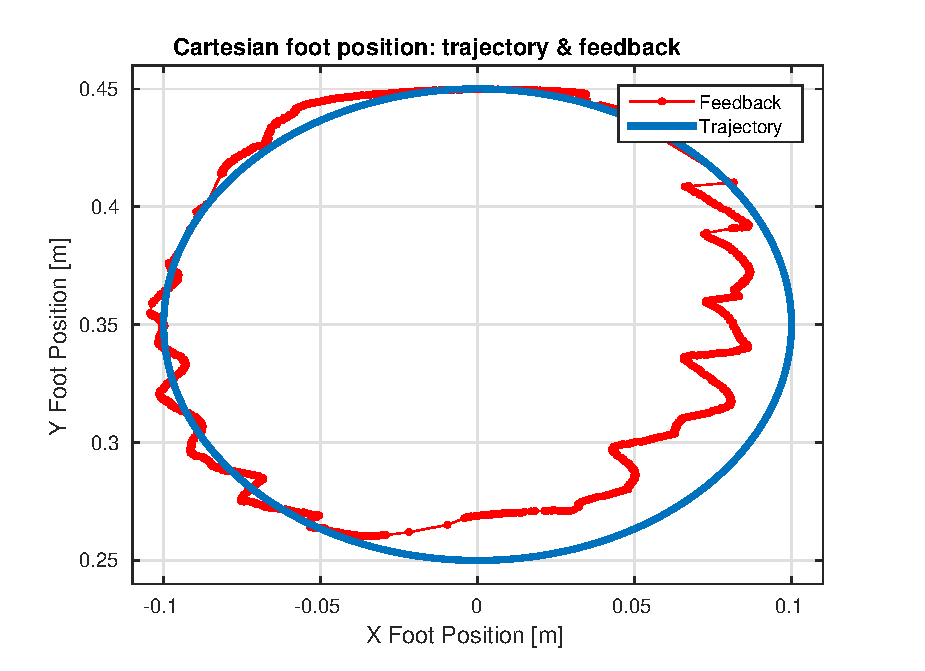
\includegraphics[width=0.5\textwidth]{images/experiments/trajectory/traj-300-5.eps}
}
\subfloat[][$K_s = 600\ N/m$; $K_d=1\ N/(m/s)$]{
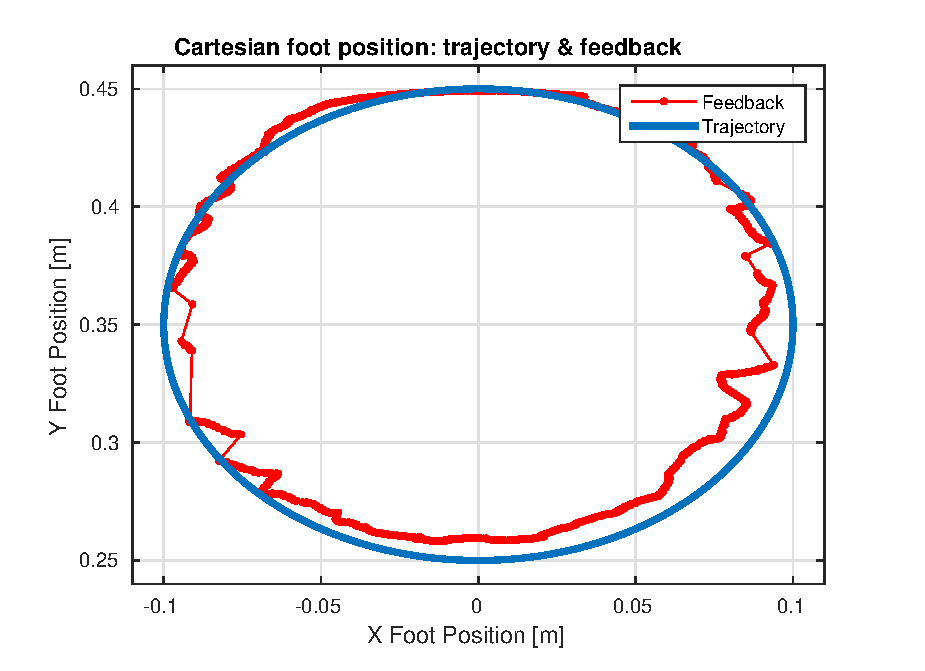
\includegraphics[width=0.5\textwidth]{images/experiments/trajectory/traj-600-1-5i.eps}
}

\subfloat[][$K_s = 600\ N/m$; $K_d=10\ N/(m/s)$]{
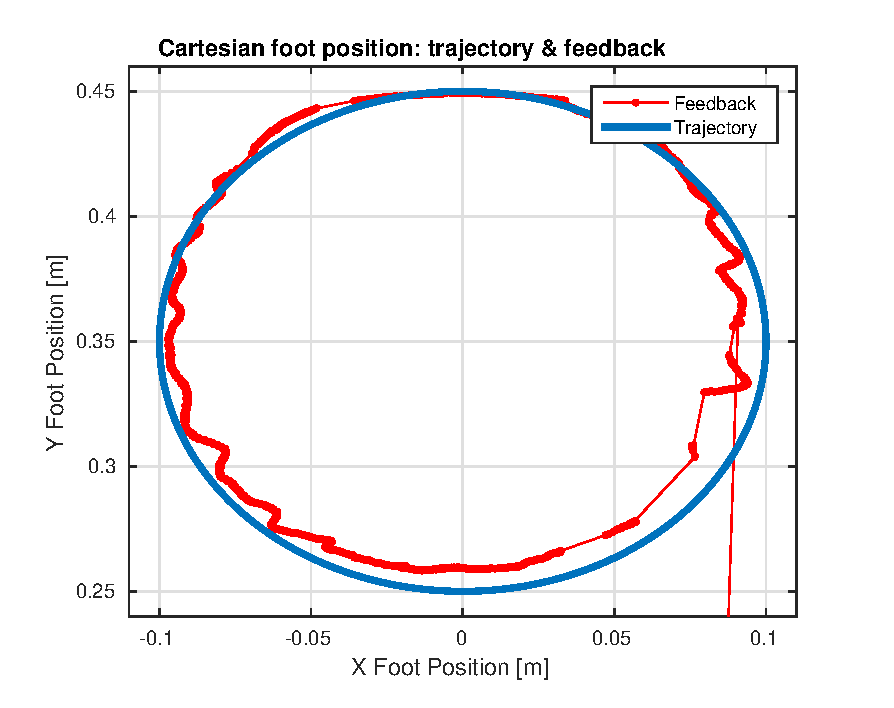
\includegraphics[width=0.5\textwidth]{images/experiments/trajectory/traj-600-10-15i.eps}
}
\subfloat[][$K_s = 600\ N/m$; $K_d=20\ N/(m/s)$]{
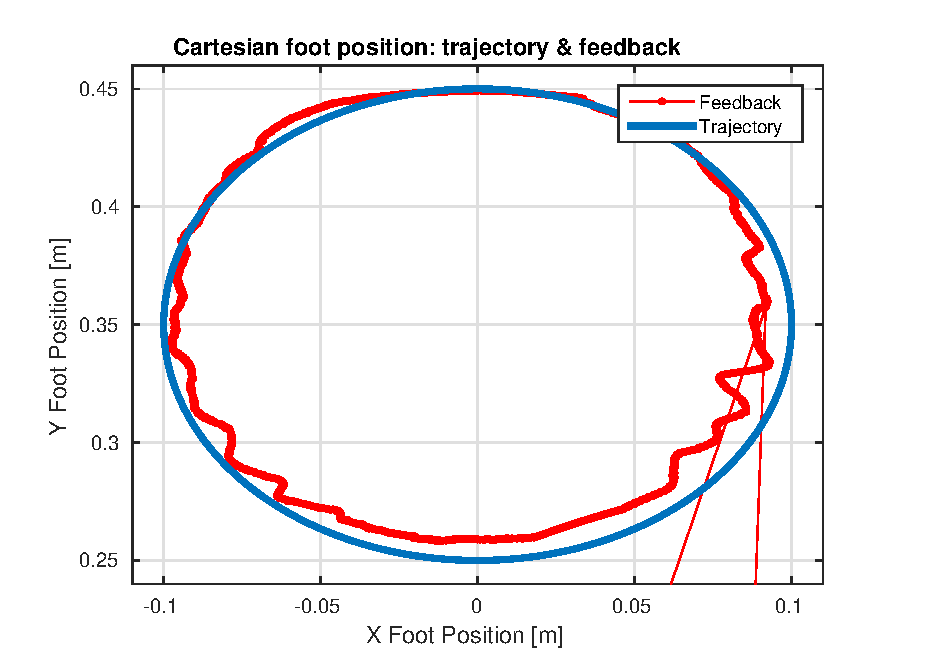
\includegraphics[width=0.5\textwidth]{images/experiments/trajectory/traj-600-20-30i.eps}
}

\subfloat[][$K_s = 800\ N/m$; $K_d=20\ N/(m/s)$]{
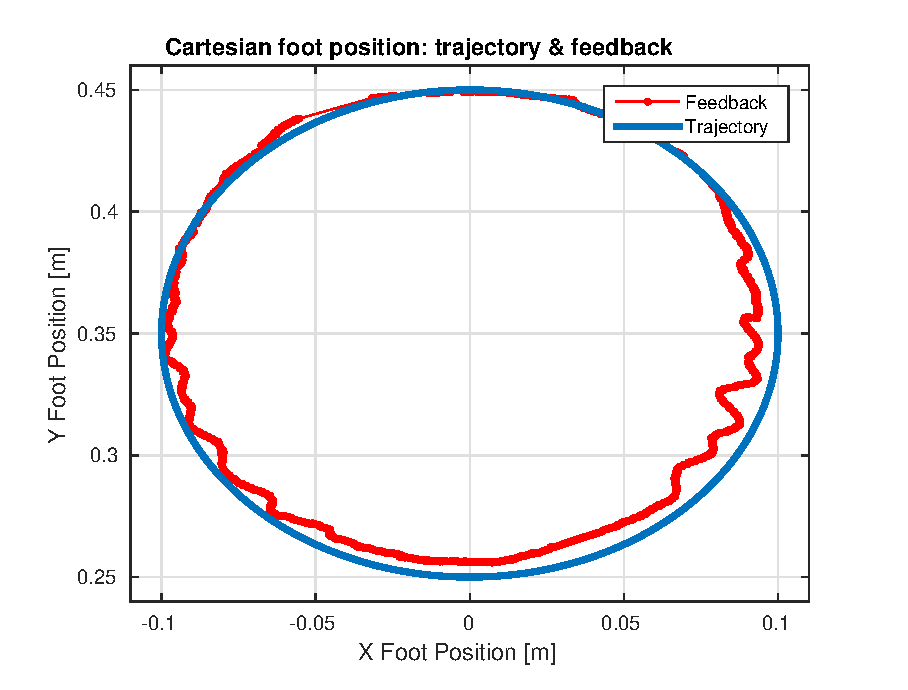
\includegraphics[width=0.5\textwidth]{images/experiments/trajectory/traj-800-20-30i.eps}
}
\subfloat[][$K_s = 1000\ N/m$; $K_d=20\ N/(m/s)$]{
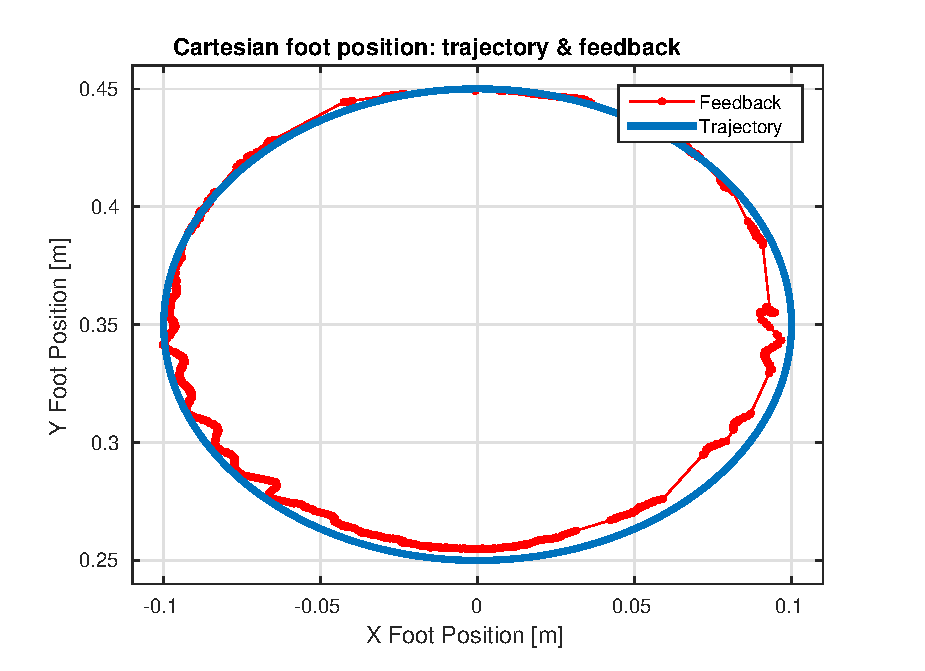
\includegraphics[width=0.5\textwidth]{images/experiments/trajectory/traj-1000-20-30i.eps}
}
\caption{Trajectory tracking for circular path to investigate effects of spring-damper constants on tracking.}
\label{fig:Trajectory tracking for circular path}
\end{figure}

\subsection{Angular Path}

An angular path was primarily chosen to investigate the linear distortion caused by a simplified kinematic mapping model. The leg model was simplified in \cref{chap:kinematics} by assuming the motors were coaxial. This makes computation more manageable on an embedded system, with the possible disadvantage of distorting the leg trajectory - this experiment aimed to test that.

The sharp angles of a square also test the leg's rapid direction changing capabilities. In the case of three dimensional movement this experiment would be critical to understanding the leg's motion during sharp turns, like in the case of a Cheetah.

The ideal spring constant for trajectory tracking, as determined in \cref{sec:Circular Path} to be $K_s = 800\ N/m$, was used, and damping constants of $K_d = 10$ and $20\ N/m$ were used along with an integral gain of $K_i = 500$.

The linear distortion can be most clearly seen along the top edge of the square, at a maximum radius of $0.45\ m$. This distortion proved to be insignificant at an error of $0.01\ m$ at its maximum at the corners. 

Asymmetry in motor movement was also discovered in the experiment. Along the right edge a relatively consistent offset of $0.01\ m$ exists. This could be caused by any number of reasons, including motor driving current loop tuning errors, or mechanical differences between leg linkages. This asymmetry can be easily corrected in the control loop by scaling  one of the motor current commands until near zero error is achieved, or until both trajectory sides match. In practise this asymmetry has little effect on leg jumping performance, but for more complex dynamic movement it should be investigated.

\begin{figure}
\centering
\subfloat[][$K_s = 800\ N/m$; $K_d=10\ N/(m/s)$; $K_i = 500$]{
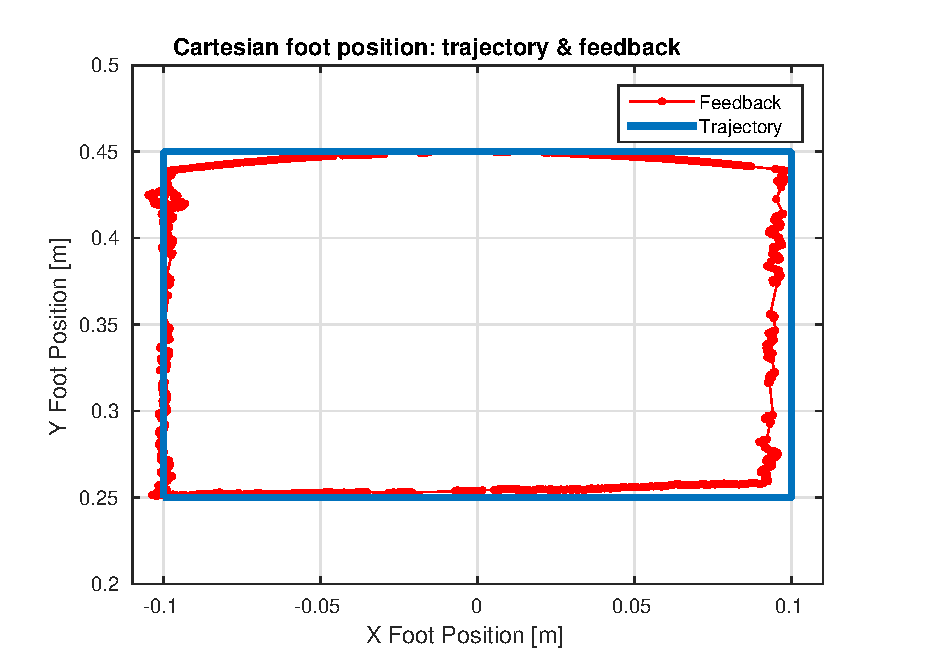
\includegraphics[width=0.5\textwidth]{images/experiments/trajectory/traj-square-800-10-500i.eps}
}
\subfloat[][$K_s = 800\ N/m$; $K_d=20\ N/(m/s)$; $K_i = 500$]{
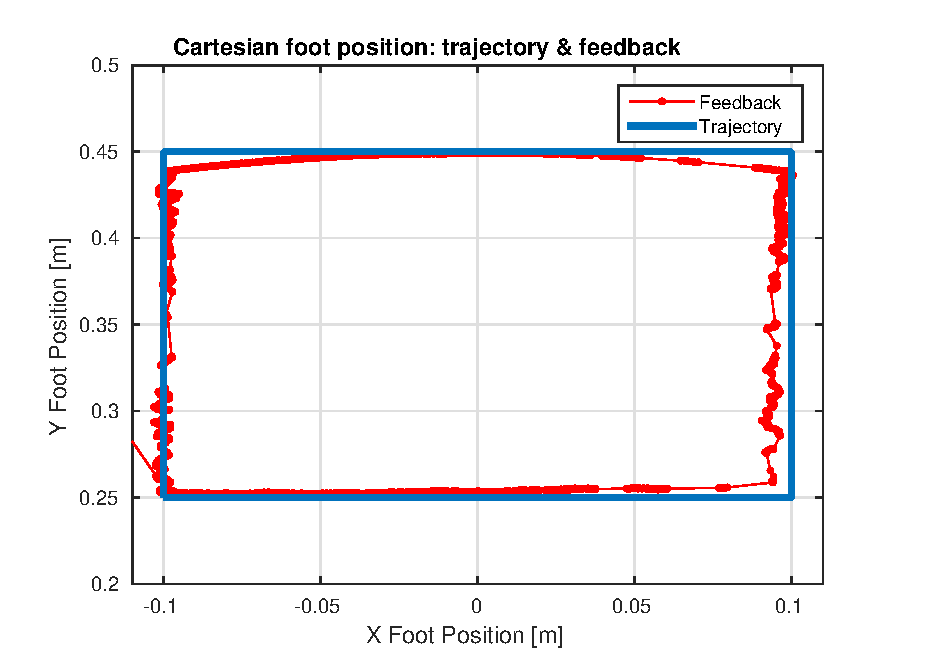
\includegraphics[width=0.5\textwidth]{images/experiments/trajectory/traj-square-800-20-500i.eps}
}
\caption{Trajectory tracking for angular path to investigate linear deformation.}
\label{fig:Trajectory tracking for angular path}
\end{figure}

\subsection{Integral Gain Trajectory Correlation}

Using the ideal spring constant for trajectory tracking, $K_s = 800\ N/m$ as determined in \cref{sec:Circular Path}, and with a damping constant of $K_d = 20\ N/m$, the experiment was performed using a circular trajectory.

Using Matlab the Pearson correlation values for the x and y Cartesian axis, $\rho_x$ and $\rho_y$, were calculated. The circular trajectory was first linearly interpolated so that the trajectory and feedback vectors for the x and y axis were of the same length. A correlation value of $\rho = 1$ indicates perfect trajectory tracking with zero error, whereas a correlation of $\rho = 0$ indicates no trajectory tracking.

In \cref{tbl:Cartesian Pearson correlation values for varying integral gain} a general upward trend in correlation can be seen for increasing integral gain. Any divergence from this trend is due to experimental error.

Integral gain clearly has a positive effect on tracking correlation and reducing steady state error. The integral error control method was only successfully implemented in this experiment after noticing the error in tracking performance. This experiment proved to validate this control method. In previous experiments for jumping and spring-damper tests the steady state error was not necessarily critical to the experiment, and even in the case of trajectory planning the error was never greater than $0.01\ m$.

The point of diminishing performance returns for integral gain was $K_i = 500$. The maximum integral gain value of $K_i = 800$ was determined based on instability in the control system for greater integral gains. Based on this we can say the ideal integral gain for stable trajectory tracking is $K_i = 500$. 

\begin{table}[]
\centering
\begin{tabular}{lll}
\textbf{$K_i$} & \textbf{$\rho_x$} & \textbf{$\rho_y$} \\
5             & 0.6716           & 0.4463           \\
10            & 0.63109          & 0.48778          \\
200           & 0.84726          & 0.632237         \\
500           & 0.86448          & 0.72518          \\
800           & 0.82182          & 0.72223         
\end{tabular}
\caption{Cartesian Pearson correlation values for a circular trajectory with varying integral gain.}
\label{tbl:Cartesian Pearson correlation values for varying integral gain}
\end{table}

\begin{figure}
\centering
\subfloat[][$K_s = 800\ N/m$; $K_d=20\ N/(m/s)$; $K_i = 5$]{
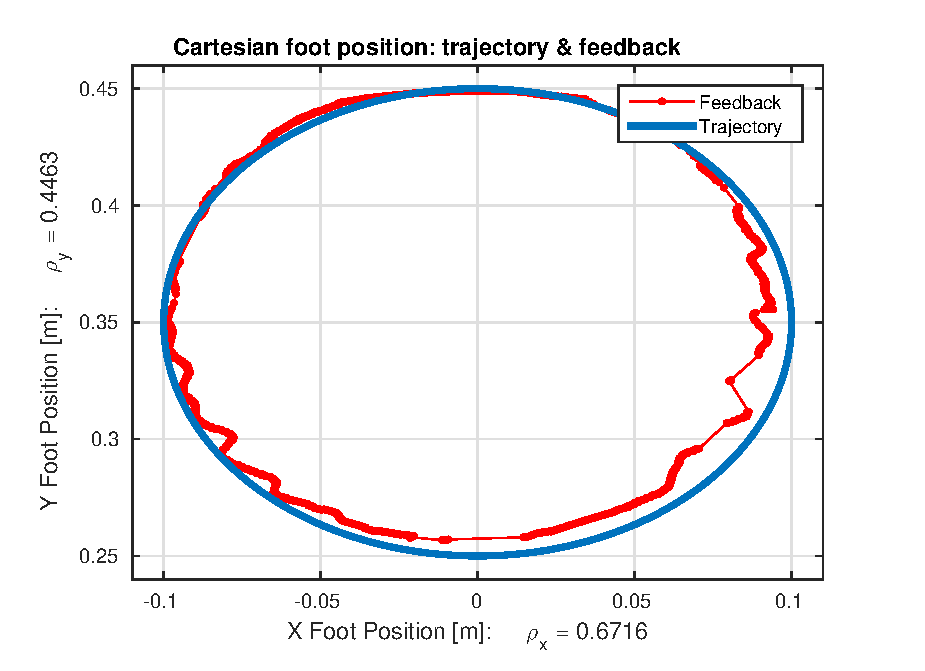
\includegraphics[width=0.5\textwidth]{images/experiments/trajectory/traj-i-5.eps}
}
\subfloat[][$K_s = 800\ N/m$; $K_d=20\ N/(m/s)$; $K_i = 10$]{
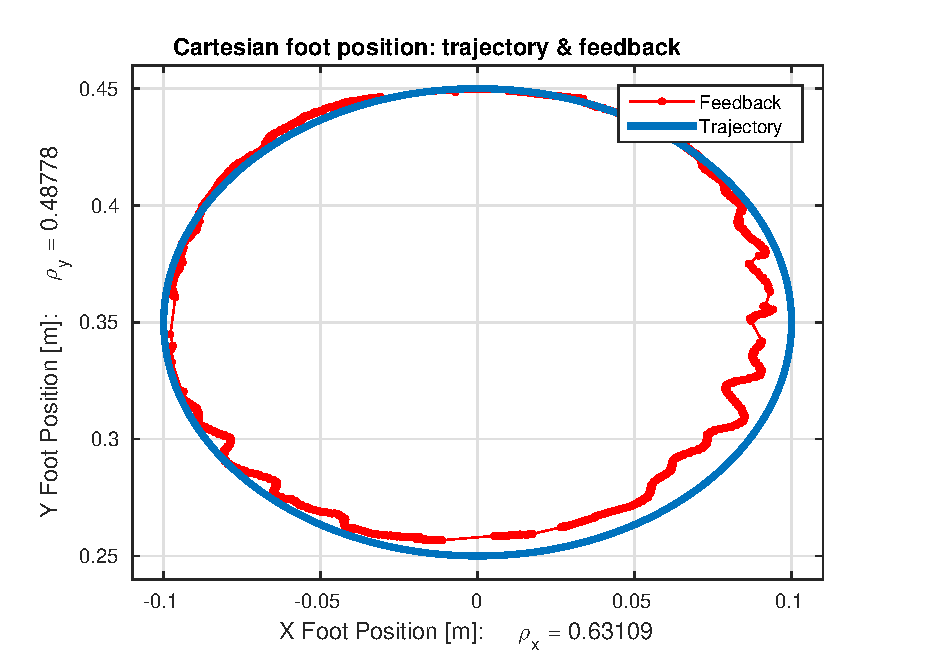
\includegraphics[width=0.5\textwidth]{images/experiments/trajectory/traj-i-10.eps}
}

\subfloat[][$K_s = 800\ N/m$; $K_d=20\ N/(m/s)$; $K_i = 200$]{
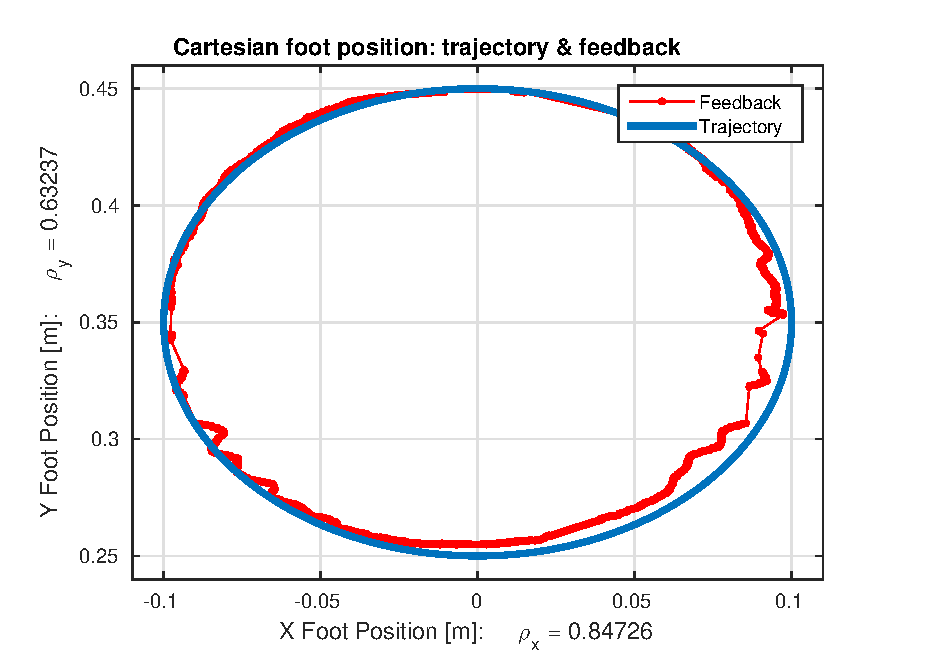
\includegraphics[width=0.5\textwidth]{images/experiments/trajectory/traj-i-200.eps}
}
\subfloat[][$K_s = 800\ N/m$; $K_d=20\ N/(m/s)$; $K_i = 500$]{
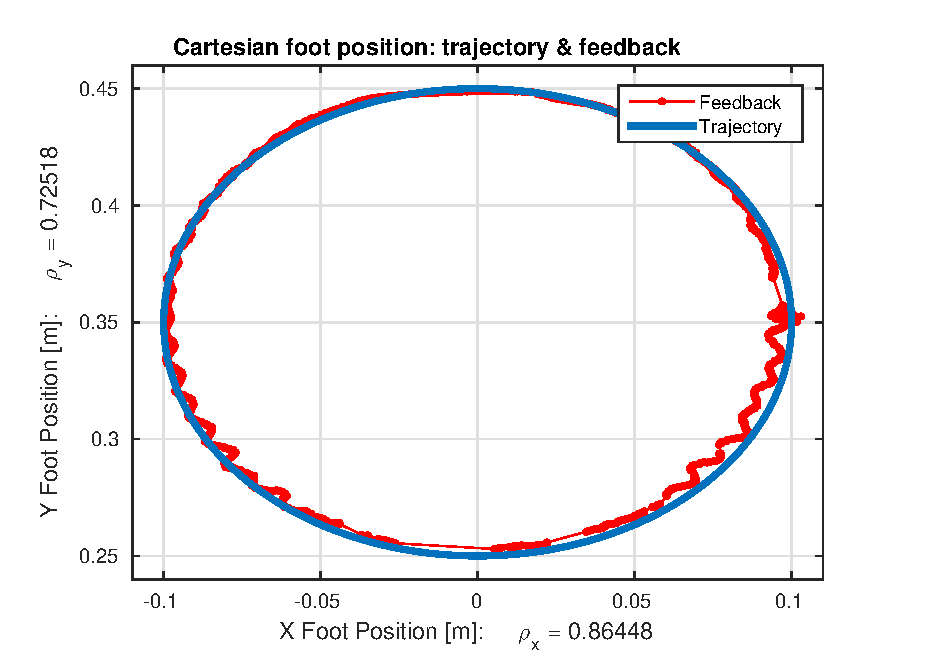
\includegraphics[width=0.5\textwidth]{images/experiments/trajectory/traj-i-500.eps}
}

\subfloat[][$K_s = 800\ N/m$; $K_d=20\ N/(m/s)$; $K_i = 800$]{
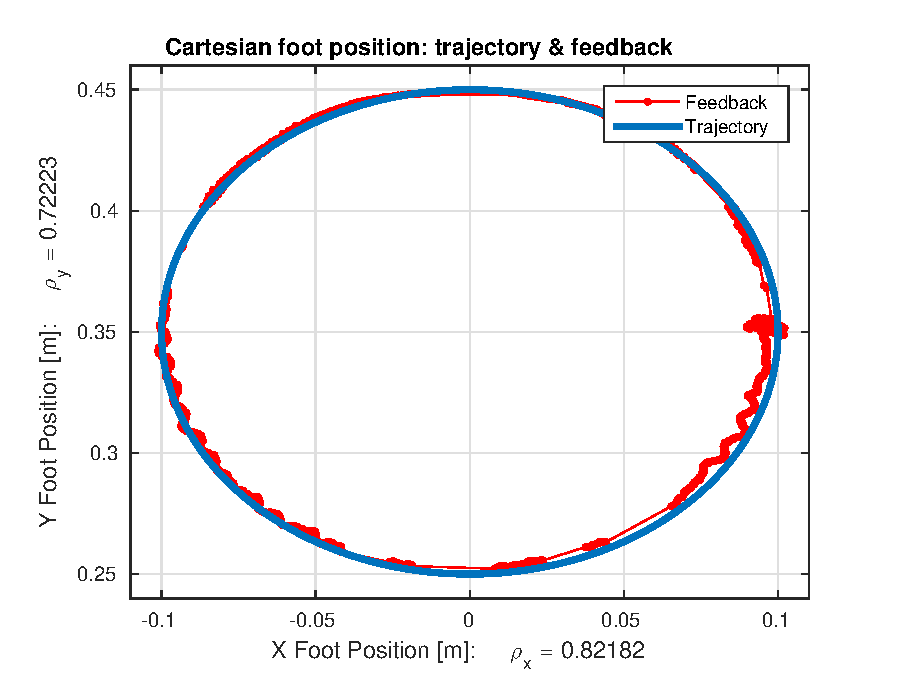
\includegraphics[width=0.5\textwidth]{images/experiments/trajectory/traj-i-800.eps}
}
\caption{Trajectory tracking for increasing integral gain with x and y correlation.}
\label{fig:Trajectory tracking for increasing integral gain}
\end{figure}

\subsection{Summary}

The following conclusions were made based on the original investigative questions:

\begin{enumerate}
\item \textbf{Effect of spring-damper constants on tracking performance, and to determine the best combination for trajectory tracking:} The spring-damper constants had minimal effect on tracking performance once the initial force deadband was overcome - this resulted in an ideal spring-damper combination of $K_s = 800\ N/m$ and $K_d = 20\ N/m$.
\item \textbf{Linear distortion caused by simplified kinematic mapping model:} The kinematic mapping model created a slight warping of the square trajectory at an extended radial set-point. This warping was insignificant at $0.01\ m$ at maximum.
\item \textbf{Effect of integral gain on tracking correlation, and to determine the best integral gain for accurate trajectory tracking while validating the integral control method:} The integral error control method was successful in reducing error in trajectory tracking. The ideal integral gain was $K_i = 800$ for stability and performance.
\item \textbf{Capability of leg to perform complex movements for three dimensional running trajectories:} The leg was capable of performing both angular and circular trajectories with considerable speed. The trajectory tracking capabilities of the leg make more complex running trajectories possible, with insignificant distortion. 
\end{enumerate}